%% ----------------------------------------------------------------
%% Thesis.tex -- MAIN FILE (the one that you compile with LaTeX)
%% ----------------------------------------------------------------

% Set up the document
\documentclass
[a4paper, 12pt, oneside]{Thesis}  % Use the "Thesis" style, based on the ECS Thesis style by Steve Gunn
\graphicspath{Figures/}  % Location of the graphics files (set up for graphics to be in PDF format)

% Include any extra LaTeX packages required
\usepackage[square, numbers, comma, sort&compress]{natbib}  % Use the "Natbib" style for the references in the Bibliography
\usepackage{verbatim}  % Needed for the "comment" environment to make LaTeX comments
\usepackage{vector}  % Allows "\bvec{}" and "\buvec{}" for "blackboard" style bold vectors in maths
\usepackage{rotating}
\usepackage{enumitem}
\usepackage{amsmath}
\usepackage{pbox}
\usepackage{hyperref}
\usepackage{pdflscape}
\usepackage{float}
\usepackage[table]{xcolor}
\usepackage{notoccite}
\usepackage{multirow}
%\usepackage{cite}
\hypersetup{urlcolor=blue, colorlinks=true}  % Colours hyperlinks in blue, but this can be distracting if there are many links.

%% ----------------------------------------------------------------
\begin{document}
\frontmatter      % Begin Roman style (i, ii, iii, iv...) page numbering

% Set up the Title Page

\title  {\vspace{+1cm}{
\includegraphics[width=30mm]{logo.pdf}}\\
\vspace{+1cm}
Development of Human-Centric Digital Twin for Industrial Applications}
%\title  {Thesis Title}}
\authors  {\texorpdfstring
            {\href{your web site or email address}{Usman Asad}}
            {Usman Asad}
            }
\addresses  {\group\\\deptname\\\univname}  % Do not change this here, instead these must be set in the "Thesis.cls" file, please look through it instead
\date       {2024}
\subject    {}

\keywords   {}

\maketitle
%% ----------------------------------------------------------------

\setstretch{1.5}  % It is better to have smaller font and larger line spacing than the other way round

% Define the page headers using the FancyHdr package and set up for one-sided printing
\fancyhead{}  % Clears all page headers and footers
\rhead{\thepage}  % Sets the right side header to show the page number
\lhead{}  % Clears the left side page header
%%%%%%%%%%%%%%%%%%%%%%%%%%%%%%%%%%%%%%%%%%%%%%%%%%%%%%%%%%%%%%%%%%%%%%%%%%%%%%%%%%%%%%%%%%%%%%%%%%%%%%%%%%%%%%%%%%%

\pagestyle{fancy}

\begin{center}
\Large{\textbf{Development of Human-Centric Digital Twin for Industrial Applications}}
\end{center}

\begin{center}
By
\\
Usman Asad\\
(DME191003)
\end{center}

\vspace{0.1cm}

\begin{center}
\textbf{Foreign Evaluator 1}\\
\textbf{University/Institute}
\end{center}

\vspace{0.5cm}

\begin{center}
\textbf{Foreign Evaluator 2}\\
\textbf{University/Institute}
\end{center}

\vspace{0.5cm}

\begin{center}
\textbf{Dr. Muhammad Mahabat Khan}\\
\textbf{(Thesis Supervisor)}
\end{center}

\vspace{0.5cm}

\begin{center}
\textbf{Dr. Muhammad Mahabat Khan}\\
\textbf{(Head, Department of Mechanical Engineering)}
\end{center}

\vspace{0.5cm}

\begin{center}
\textbf{Dr. Imtiaz Ahmad Taj}\\
\textbf{(Dean, Faculty of Engineering)}
\end{center}

\vspace{2cm}

\begin{center}
\textbf{DEPARTMENT OF MECHANICAL ENGINEERING\\
CAPITAL UNIVERSITY OF SCIENCE AND TECHNOLOGY\\
ISLAMABAD\\
2024}
\end{center}

\clearpage


\pagestyle{fancy}

\begin{center}
\large{Copyright \copyright~2024 by Usman Asad}
\end{center}

All rights reserved. No part of this thesis may be reproduced, distributed, or transmitted in any form or by any means, including photocopying, recording, or other electronic or mechanical methods, by any information storage and retrieval system without the prior written permission of the author.

\clearpage
%%%%%%%%%%%%%%%%%%%%%%%%%%%%%%%%%%%%%%%%%%%%%%%%%%%%%%%%%%%%%%%%%%%%%%%%%%%%%%%%%%%%%%%%%%%%%%%%%%

\pagestyle{fancy}  % No headers or footers for the following pages

\null\vfill\vfill\vfill\vfill\vfill
% Now comes the "Funny Quote", written in italics
\begin{center}
	\LARGE{\textit{Write dedication here}}
\end{center}

\vfill\vfill\vfill\vfill\vfill\vfill\null
%
\clearpage

\pagestyle{fancy}

\null\vfill\vfill\vfill\vfill\vfill
% Now comes the "Funny Quote", written in italics
\begin{center}
	\LARGE{\textit{This page is left blank for HEC certificate}}
\end{center}

\vfill\vfill\vfill\vfill\vfill\vfill\null

\clearpage

%%%%%%%%%%%%%%%%%%%%%%%%%%%%%%%%%%%%%%%%%%%%%%%%%%%%%%%%%%%%%%%%%%%%%%%%%%%%%%%%%%%%%%%%%%%%%%%%%%%%%%%%%%
\pagestyle{fancy}
%\lhead{List of Tables}  % Set the left side page header to "List of Tables"
\addtotoc{Author's Declaration}
\declaration{
\addtocontents{toc}{{\vspace{0.5em}}}

I, \textbf{Usman Asad} hereby state that my PhD thesis titled ``\textbf{Development of Human-Centric Digital Twin for Industrial Applications}" is my own work and has not been submitted previously by me for taking any degree from Capital University of Science and Technology, Islamabad or anywhere else in the country/abroad.

At any time if my statement is found to be incorrect even after my graduation, the University has the right to withdraw my PhD Degree.

\vspace{2cm}

\textbf{(Usman Asad)}\\
Registration No:~DME191003
}

%% ----------------------------------------------------------------
\clearpage
%% %%%%%%%%%%%%%%%%%%%%%%%%%%%%%%%%%%%%%%%%%%%%%%%%%%%%%%%%%%%%%%%%%%%%%%%%%%%%
\pagestyle{fancy}
%\lhead{List of Tables}  % Set the left side page header to "List of Tables"
\addtotoc{Plagiarism Undertaking}
\plagiarism{
\addtocontents{toc}{{\vspace{0.5em}}}


I solemnly declare that research work presented in this thesis titled ``\textbf{Development of Human-Centric Digital Twin for Industrial Applications}" is solely my research work with no significant contribution from any other person. Small contribution/help wherever taken has been duly acknowledged and that complete thesis has been written by me.

I understand the zero tolerance policy of the HEC and Capital University of Science and Technology towards plagiarism. Therefore, I as an author of the above titled thesis declare that no portion of my thesis has been plagiarized and any material used as reference is properly referred/cited.

I undertake that if I am found guilty of any formal plagiarism in the above titled thesis even after award of PhD Degree, the University reserves the right to withdraw/revoke my PhD degree and that HEC and the University have the right to publish my name on the HEC/University website on which names of students are placed who submitted plagiarized work.

\vspace{2cm}

\textbf{(Usman Asad)}\\
Registration No:~DME191003
}
\clearpage
%%%%%%%%%%%%%%%%%%%%%%%%%%%%%%%%%%%%%%%%%%%%%%%%%%%%%%%%%%%%%%%%%%%%%%%%%%%%%%%%%%%%%%%%%%%%%%%%%
\pagestyle{fancy}
%\lhead{List of Tables}  % Set the left side page header to "List of Tables"
\addtotoc{List of Publications}
\publications{
\addtocontents{toc}{{\vspace{0.5em}}}

It is certified that following publication(s) have been made out of the research work that has been carried out for this thesis:-

\begin{enumerate}
    \item \textbf{U. Asad}, M. M. Khan, A. Khalid, W. A. Lughmani, and S. Rasheed, ``A human intention and motion prediction framework for applications in human-centric digital twins," \textit{Biomimetics}, submitted for publication.
    
    \item \textbf{U. Asad}, M. Khan, A. Khalid, and W. A. Lughmani, ``Human-centric digital twins in industry: A comprehensive review of enabling technologies and implementation strategies," \textit{Sensors}, vol. 23, no. 8, p. 3938, 2023.

    
\end{enumerate}

\vspace{2cm}

\textbf{(Usman Asad)}\\
Registration No:~DME191003


}
\clearpage
%%%%%%%%%%%%%%%%%%%%%%%%%%%%%%%%%%%%%%%%%%%%%%%%%%%%%%%%%%%%%%%%%%%%%%%%%%%%%%%%%%%%%%%%%%%%%%%%%%%%%%%%%%%%%%%%%%%%%%%%%%%%%%%%%%%%%%%%%%%%%%
\pagestyle{fancy}
%\lhead{List of Tables}  % Set the left side page header to "List of Tables"
\addtotoc{Acknowledgement}
\acknowledgement{
\addtocontents{toc}{{\vspace{0.5em}}}

Write your acknowledgement here

\vspace{2cm}

\textbf{(Your Name)}

}
\clearpage  % End of the Acknowledgements

%%%%%%%%%%%%%%%%%%%%%%%%%%%%%%%%%%%%%%%%%%%%%%%%%%%%%%%%%%%%%%%%%%%%%%%%%%%%%%%%%%%%%%%%%%%%%%%%%%%%%%%%%%%%%%%%%%%%%%%%%%%%%%%%%%%%%%%%%%%%%%%%
% The Abstract Page
\addtotoc{Abstract}  % Add the "Abstract" page entry to the Contents
\abstract{
\addtocontents{toc}{\vspace{0.5em}}  % Add a gap in the Contents, for aesthetics

In the evolution towards Industry 5.0, the focus on human-centricity is paramount, transforming industrial workspaces into collaborative environments where humans and robots operate in synergy. However, conventional digital twins often neglect the crucial human element, limiting the potential for truly intelligent and safe Human-Robot Collaboration (HRC). A significant challenge remains in creating systems that can proactively anticipate human actions to enable seamless and safe task execution. Current foundation models, despite their advanced reasoning capabilities, often fall short in translating high-level semantic understanding into the accurate, context-aware prediction of complex human motion required for proactive assistance. This gap hinders the transition of robotic assistants from reactive tools to intelligent, symbiotic partners.

This thesis addresses this challenge by developing and validating a modular Human-Centric Digital Twin (HCDT) framework designed to predict human intention and forecast plausible future motion. The proposed framework integrates state-of-the-art pre-trained modules, comprising: a perception module for robust human pose and gaze estimation; an AI-driven reasoning module that leverages Vision-Language Models (VLMs) to interpret multi-modal context and predict task state and future hand positions; and a motion generation module that synthesizes physically plausible, full-body 3D motion trajectories. By structuring task knowledge and engineering context-rich prompts, the framework guides VLMs to achieve nuanced intention understanding in semi-structured environments.


The framework's performance was systematically evaluated across three use cases of varying complexity, including assembly and domestic tasks. The evaluation reveals a critical trade-off between prediction accuracy and latency. A proposed Rolling Context Window (RCW) strategy, which utilizes a history of frames and the previously predicted state, is shown to achieve a strong balance of performance and efficiency, significantly outperforming single-image and computationally expensive in-context learning methods. Furthermore, the results demonstrate that incorporating egocentric video views yields a substantial $10.7\%$ performance increase in complex scenarios, and that short-term motion forecasting is significantly enhanced by conditioning on historical pose, gaze data, and in-context examples.


Ultimately, this research contributes a scalable and practical framework that bridges high-level semantic reasoning with physically grounded motion synthesis. By enabling more accurate prediction of human intent and motion, this work advances the development of intelligent HCDTs, paving the way for safer, more efficient, and truly symbiotic human-robot collaboration in next-generation manufacturing environments.


}
\clearpage  % Abstract ended, start a new page
%% ----------------------------------------------------------------

%% ----------------------------------------------------------------

\pagestyle{fancy}  %The page style headers have been "empty" all this time, now use the "fancy" headers as defined before to bring them back


%% ----------------------------------------------------------------
\tableofcontents  % Write out the Table of Contents

%% ----------------------------------------------------------------
\listoffigures  % Write out the List of Figures

%% ----------------------------------------------------------------
\listoftables  % Write out the List of Tables

%% ----------------------------------------------------------------
\setstretch{1.5}  % Set the line spacing to 1.5, this makes the following tables easier to read
\clearpage  % Start a new page
\listofsymbols{ll}  % Include a list of Abbreviations (a table of two columns)
{
% \textbf{Acronym}  & \textbf{W}hat (it) \textbf{S}tands \textbf{F}or \\
\textbf{AI} & Artificial Intelligence \\
\textbf{AR} & Augmented Reality \\
\textbf{BT} & Behavior Tree \\
\textbf{DAG} & Directed Acyclic Graph \\
\textbf{GVHMR} & Global-View Human Mesh Recovery \\
\textbf{HCDT} & Human-Centric Digital Twin \\
\textbf{HMLV} & High-Mix, Low-Volume \\
\textbf{HRC} & Human-Robot Collaboration \\
\textbf{ICL} & In-Context Learning \\
\textbf{KG} & Knowledge Graph \\
\textbf{LLM} & Large Language Model \\
\textbf{ML} & Machine Learning \\
\textbf{MoCap} & Motion Capture \\
\textbf{NMPE} & Normalized Mean Position Error \\
\textbf{PDDL} & Planning Domain Definition Language \\
\textbf{POI} & Point of Interest \\
\textbf{RCW} & Rolling Context Window \\
\textbf{SME} & Small and Medium Enterprises \\
\textbf{SMPL-X} & Skinned Multi-Person Linear Model with Extensions \\
\textbf{TSA} & Task State Accuracy \\
\textbf{VLM} & Vision-Language Model \\
\textbf{VR} & Virtual Reality \\
}

%% ----------------------------------------------------------------
%\clearpage  % Start a new page
%\listofconstants{lrcl}  % Include a list of Physical Constants (a four column table)
%{
%% Constant Name & Symbol & = & Constant Value (with units) \\
%Speed of Light & $c$ & $=$ & $2.997\ 924\ 58\times10^{8}\ \mbox{ms}^{-\mbox{s}}$ (exact)\\
%
%}

%% ----------------------------------------------------------------
\clearpage  %Start a new page
\listofnomenclature{lll}  % Include a list of Symbols (a three column table)
{
% symbol & name & unit \\
$\mathcal{V}$ & History of video frames \\
$\mathcal{P}$ & History of extracted human poses \\
$\mathcal{C}_{task}$ & Static, high-level task knowledge \\
$\mathcal{F}$ & Framework function for prediction \\
$S_t$ & Predicted task state at time $t$ \\
$\hat{H}_{t+\Delta t}$ & Forecast of future hand positions \\
$\hat{M}_{t_i}$ & Predicted full-body 3D motion trajectory \\
$N_{\text{pred}}$ & Number of predicted frames in a motion trajectory \\
$I_k$ & Video frame at a specific time step $k$ \\
$P_k$ & Human pose at a specific time step $k$ \\

% SMPL-X and Pose Symbols
$\boldsymbol{\beta}$ & SMPL-X body shape parameters \\
$\boldsymbol{\theta}$ & SMPL-X body pose parameters \\
$\boldsymbol{\psi}$ & SMPL-X expressive hand and face parameters \\
$R_{wc}$ & Rotation matrix from world to camera frame \\
$\mathbf{t}_{wc}$ & Translation vector from world to camera frame \\
$\mathbf{x}_c$ & 3D point in camera coordinates \\
$\mathbf{x}_w$ & 3D point in world coordinates \\

% Motion and Kinematic Symbols
$D(\cdot, \cdot)$ & Euclidean distance function \\
$\mathbf{p}_{\text{pred}}$ & Predicted position vector for Prediction Diversity \\
$\bar{\mathbf{p}}_{\text{in}}$ & Average position of the input trajectory \\
$\mathbf{p}_{\text{last}}$ & Last position in the input trajectory \\
}
%% ----------------------------------------------------------------
% End of the pre-able, contents and lists of things
% Begin the Dedication page

%\setstretch{1.3}  % Return the line spacing back to 1.3
%
%\pagestyle{empty}  % Page style needs to be empty for this page
%\dedicatory{To those who works for humanity...\ldots}
%
%\addtocontents{toc}{\vspace{2em}}  % Add a gap in the Contents, for aesthetics


%% ----------------------------------------------------------------
\mainmatter	  % Begin normal, numeric (1,2,3...) page numbering
\pagestyle{fancy}  % Return the page headers back to the "fancy" style

% Include the chapters of the thesis, as separate files
% Just uncomment the lines as you write the chapters
\lhead{\emph{Introduction}}  % Set the left side page header to "Contents"
\chapter{Introduction}
\label{chap:introduction}

\section{Background}
\label{sec:background}

The manufacturing landscape is undergoing a significant transformation, moving from the technology-driven paradigm of Industry 4.0 to the value-driven, human-centric principles of Industry 5.0. This evolution emphasizes a synergistic union between human capabilities and robotic systems, fostering collaborative workspaces where people and machines operate in close proximity. This shift is driven by the realization that full automation is not always the most effective solution, especially in high-mix, low-volume (HMLV) production environments that demand flexibility, creativity, and complex problem-solving—qualities inherent to human workers. The concept of Human-Robot Collaboration (HRC) is central to this new era, aiming to combine human ingenuity and dexterity with the precision, repeatability, and strength of robots.

To facilitate this deeper integration, the concept of the Digital Twin (DT)—a virtual replica of a physical asset or system—has been extended to include the human element, leading to the emergence of the Human-Centric Digital Twin (HCDT). An HCDT is a dynamic virtual model of a human operator, integrating data on their physical state, behavior, and even cognitive load. The goal of an HCDT is to create a symbiotic relationship where the robotic system can understand, anticipate, and adapt to the human's needs, enhancing safety, ergonomics, and overall productivity.

Recent advancements in Artificial Intelligence (AI), particularly in computer vision, sensor technology, and machine learning, have provided the foundational tools to build these sophisticated HCDTs. Vision-Language Models (VLMs) and other foundation models have demonstrated remarkable capabilities in semantic understanding and reasoning, opening new avenues for robots to interpret complex, unstructured human actions. This research is situated at the intersection of these fields, exploring how to leverage these technological strides to create truly intelligent and proactive robotic partners. A key application area with significant potential for HRC is composites manufacturing, a traditionally labor-intensive process involving the manipulation of deformable materials, which presents unique challenges for automation.

\section{Limitations of Current Approaches}
\label{sec:limitations}

Despite the rapid technological progress, several critical limitations hinder the widespread adoption of truly collaborative and intelligent robotic systems.

\begin{enumerate}
    \item Neglect of the Human Element in Digital Twins: A comprehensive review of existing literature reveals that the vast majority of DT implementations focus almost exclusively on the physical assets (machines, production lines) of a Cyber-Physical System. The human operator is often overlooked or modeled in a simplistic, static manner. This system-centric view fails to capture the dynamic and nuanced nature of human behavior, limiting the robot's ability to adapt and collaborate effectively.

    \item Challenges in Human Intent and Motion Prediction: For a robot to be a proactive partner, it must be able to anticipate what a human intends to do next. However, predicting human intent is a formidable challenge. Human actions are often stochastic, context-dependent, and driven by complex internal states. Current models struggle to translate high-level semantic understanding into accurate, granular predictions of future 3D human motion, especially over long horizons. This results in reactive, rather than proactive, robotic assistance.

    \item Rigidity of Automation in Complex Tasks: Traditional robotic programming is ill-suited for the dynamic and variable nature of HMLV manufacturing and tasks involving deformable materials, such as composite layup. These tasks require adaptability and fine motor skills that are difficult to encode in rigid, pre-programmed routines. While learning-from-demonstration methods show promise, they often require extensive data and struggle to generalize to novel situations.

    \item The Sim-to-Real Gap: While simulation is a powerful tool for developing and training robotic systems, a significant gap often exists between the simulated environment and the real world. This is particularly true for modeling the complex physics of deformable materials and the unpredictable nature of human interaction, making it difficult to transfer learned policies reliably to physical robots.
\end{enumerate}

\section{Problem Statement}
\label{sec:problem_statement}

The central problem addressed by this thesis is the gap between the conceptual promise of human-centric manufacturing and the practical limitations of current robotic systems. Specifically, existing frameworks lack the capability to robustly predict human intention and forecast detailed, physically plausible future motion in a way that enables proactive and intelligent robotic assistance in complex, semi-structured tasks. This deficiency prevents robots from transitioning from simple collaborative tools into truly symbiotic partners that can anticipate needs, pre-empt actions, and enhance human capabilities.

Therefore, this research aims to develop and validate a modular Human-Centric Digital Twin (HCDT) framework that can accurately predict human intention and generate context-aware, full-body 3D motion forecasts to enable proactive robotic assistance in manufacturing environments, with a specific focus on the challenges presented by deformable object manipulation in composites manufacturing.

\section{Research Objectives}
\label{sec:objectives}

To address the problem statement, this thesis pursues the following specific objectives:

\begin{enumerate}
    \item To develop a modular and scalable HCDT framework that integrates state-of-the-art, pre-trained AI modules for perception, reasoning, and motion generation, minimizing the need for extensive task-specific training.

    \item To investigate and implement novel strategies for human intention prediction by leveraging Vision-Language Models (VLMs) to interpret rich, multi-modal context from video streams, task knowledge graphs, and human gaze data.

    \item To create a robust pipeline for generating physically plausible, full-body 3D human motion forecasts that are conditioned on the predicted intent, enabling the visualization and simulation of future actions within the digital twin.

    \item To apply and validate the developed framework on a challenging industrial use case: the manual layup of composite materials. This involves creating a specialized digital twin for deformable object manipulation and demonstrating how the framework can enhance this process.

    \item To demonstrate the framework's capability to enable proactive robotic assistance, showing how the predictive outputs of the HCDT can be used to inform a robot's actions, allowing it to provide timely and effective support to a human operator.

    \item To systematically evaluate the performance of the framework across multiple use cases of varying complexity, establishing benchmarks and identifying the trade-offs between prediction accuracy, latency, and contextual richness.
\end{enumerate}

\section{Thesis Layout}
\label{sec:layout}

This thesis is structured into six chapters, each building upon the previous one to present a comprehensive body of research.

\begin{itemize}
    \item Chapter 1: Introduction. This chapter provides the background and motivation for the research, outlines the limitations of current approaches, defines the problem statement and research objectives, and presents the overall structure of the thesis.

    \item Chapter 2: Human-centric Digital Twins in Industry: Enabling Technologies and Implementation Strategies. This chapter presents a comprehensive literature review, establishing the theoretical foundation for the research. It surveys the state-of-the-art in HCDTs, HRC, AI-driven motion prediction, and the enabling technologies that underpin these fields.

    \item Chapter 3: Human Intention and Motion Prediction Framework. This chapter details the core contribution of the thesis: the design and architecture of the proposed modular HCDT framework. It describes the individual components for perception, AI-driven reasoning, and motion generation, and explains how they are integrated to achieve intent-aware motion forecasting.

    \item Chapter 4: Development of Digital Twin for Composite Layup. This chapter focuses on the first major application and validation of the framework. It details the development of a specialized digital twin for the complex task of composites manufacturing, addressing the specific challenges of modeling and simulating deformable materials and the associated human-robot interactions.

    \item Chapter 5: Proactive Robotic Assistance in HCDTs. Building on the predictive capabilities developed in the previous chapters, this chapter demonstrates how the HCDT's outputs can be used to drive a physical or simulated robot. It presents experiments showing how the robot can provide proactive assistance to a human operator, validating the practical utility of the framework.

    \item Chapter 6: Conclusion and Future Work. The final chapter summarizes the key findings and contributions of the thesis. It reflects on the achievement of the research objectives, discusses the broader implications of the work, acknowledges its limitations, and proposes promising directions for future research.
\end{itemize} % Introduction
\clearpage
\lhead{\emph{Overview of Human-centric Digital Twins}}  % Set the left side page header to "Contents"
\chapter{Overview of Human-centric Digital Twins}
\label{chap:literature_review}

\section{Introduction}

Industry has a constant need to evolve, innovate and adopt technological advances in order to meet the challenges of the future in a competitive environment. Broadly in literature, historical industrial progress is divided into epochs called "Industrial Revolutions", characterized by major technological paradigm shifts \cite{Nahavandi2019}. In light of the digital revolution and exponential growth in computational power, information and data processing capabilities, smart sensors, and computational intelligence, the focus of Industry 4.0, is to leverage emerging technologies to interconnect smart Cyber-Physical Systems (CPS) to enable mass-customization in robust flexible Smart Factories. A synergistic paradigm of emerging technologies is recently developing, which includes leveraging multi-physics simulations to create Digital Twins (DT) of physical systems. DTs use immersive technologies such as Virtual Reality (VR) and Augmented Reality (AR) to explore and interact with virtual objects, and using Collaborative Robots for safe, intuitive Human-Robot Interaction (HRI), especially by utilizing advances in Artificial Intelligence. There is an increasing realization that in addition to technological aspirations, government, and Industry should move towards a value-driven future where the focus is on human well-being, sustainability, and resilience under Industry 5.0 \cite{Lu-ManuOutlook}.

\subsection{Cyber-Physical Systems and Digital Twins}
In the context of Industry 4.0, certain enabling technologies such as distributed computing, sensor networks, big data, and the Internet of Things (IoT) have found increasing application in manufacturing settings to achieve reliability, flexibility, increased automation, and better performance \cite{Gallala2022}. Due to advances in computational intelligence, increasing data bandwidth and processing capability, and widespread use of sensors, it has become possible to create highly autonomous virtual replicas of CPS with advanced decision-making capabilities. These highly autonomous virtual replicas are known as Digital Twins. The term 'Digital Twin' is popularized by NASA in the context of flying vehicles \cite{shafto2012modeling}. Many definitions of DTs have been proposed in literature. The definition proposed by AIAA \cite{AIAA} is "A set of virtual information constructs that mimic the structure, context, and behavior of an individual/unique physical asset, or a group of physical assets, is dynamically updated with data from its physical twin throughout its life cycle and informs decisions that realize value".

Although the concept of DTs originated from the aerospace industry, it can now be used for the digital representation of any complex system \cite{Ammar2022}. DTs have been employed in many traditional manufacturing areas including metallurgy, machining, grinding, and hole punching \cite{Liu2021-Review}. Functionally, DTs are used for supervision, interaction, and prediction of assets, often exploiting Artificial Intelligence and immersive user experience, for example using Extended Reality (XR) \cite{Turner2022}.

\subsection{Human Robot Collaboration}
Industrial Robots driven by Programmable Logical Controllers executing fixed sets of instructions have become a staple of automation and mass production in advanced factories. Most such Industrial Robots are entirely separated from human workers through safety fencing or large distances. Increasingly, there is a trend towards re-introducing human workers to the factory floor to work side-by-side with collaborative robots (Cobots). The coexistence of humans and Cobots leverages human creativity and general intelligence, as well as robot precision and repeatability and highly increased perception due to rapid developments in Artificial Intelligence technologies. Emerging avenues in Human-Robot Collaboration (HRC) focus on human centricity, where a more symbiotic relationship between humans and robots is envisioned, where human performance and perception can be enhanced by using Exoskeletons, Cognitive Ability, Co-Intelligence, Mixed Reality, and Brain-Computer Interface (BCI) \cite{Wang-FuturePerspective-2022}.

\subsection{Human-Centric Digital Twins}
Human centricity is an important hallmark of "Industry 5.0", which is envisioned to be a value-based Industrial Revolution with a focus on human well-being, sustainability, flexibility, and efficiency \cite{Xu2021}. This comes with the realization that the objective of automation is not the elimination of labor altogether, but to leverage the creativity, objective thinking, dexterity, and decision-making power of humans alongside the repeatability, accuracy, and convenience of using robots for repetitive, labor-intensive, tedious tasks \cite{Land2020}. This gives rise to the idea of Operator 5.0 \cite{Wang2022-HCPSPerspective}, where human perception, cognition, and interaction capabilities are enhanced by a range of enabling technologies, as shown in Figure \ref{figure:Ov4}.

\begin{figure}[h]
    \centering
    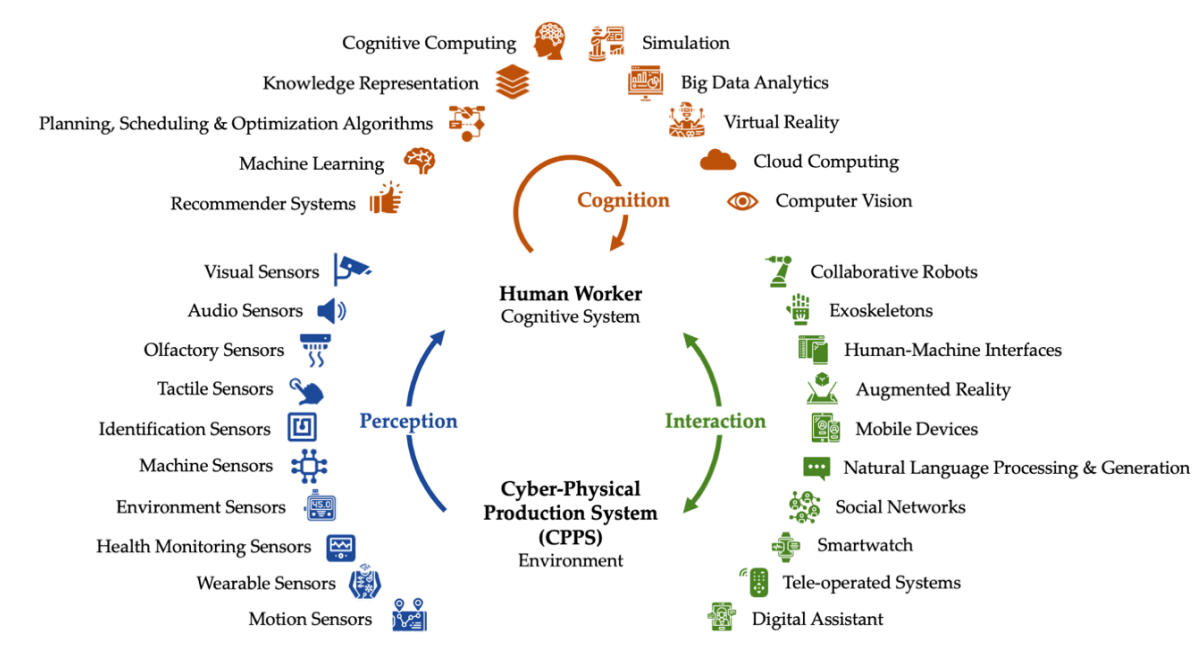
\includegraphics[width=0.8\linewidth]{ThesisFigs/Lando.png}
    \caption{Symbiotic human-machine relationship in Industry 5.0 \cite{Longo2020}}
    \label{figure:Ov4}
\end{figure}

In order to better integrate humans in CPS, the concept of Human Digital Twins is finding increasing popularity, in order to better monitor, evaluate and optimize human performance, ergonomics and well-being \cite{Locklin2021}. Development of Human Digital Twins involves the deployment of a model of humans using sensor data which provides insight into their behavior and attributes, which may include their physical, physiological, cognitive, and emotional states \cite{Miller2022}. Creating a symbiotic human-robot collaboration system requires the use of dynamic monitoring of humans and resources using smart sensors, active collision avoidance, dynamic planning, and context-aware adaptive robot control \cite{Wang2019}.

\section{Human Intent and Motion Prediction}
A truly effective Human-Centric Digital Twin (HCDT) must go beyond simply monitoring the current state of a human operator; it must be able to anticipate their future actions. This predictive capability is paramount for robots to transition from reactive assistance to proactive, intelligent collaboration \cite{Asad_Intention_2025}. The endeavor to create such proactive robotic assistants draws upon several interconnected research areas, including human intent prediction, AI-driven motion generation, and the application of Large Language Models (LLMs) to robotics.

\subsection{Human Intent Prediction for Collaborative Environments}
Anticipating human intent is pivotal to enhancing safety, ergonomics, and effective collaboration in Industry 5.0. Early work often focused on trajectory prediction in constrained scenarios \cite{Huang2021}. More recent approaches have sought to infer higher-level goals. For instance, Huang et al. \cite{Huang2022} proposed a hierarchical intention-tracking framework for assembly tasks, utilizing OpenPose and Kalman filtering to track wrist positions and infer both high-level task goals and low-level current actions. Similarly, Mangin et al. \cite{Mangin2022} developed hierarchical planners that infer human goals using partially observable Markov decision processes for procedural tasks. The use of egocentric data has also gained traction, with works like Mascaro et al. \cite{Mascaro2022} developing intention-conditioned hierarchical architectures for long-term action anticipation. However, many existing methods focus on recognizing intent from past actions rather than proactively forecasting future motion linked to that intent.

\subsection{AI-Driven Virtual Human Motion Generation}
Generating realistic and controllable human motion is a long-standing challenge. The field has historically relied on motion capture (MoCap) datasets, which provide high-fidelity kinematic data. A significant advancement was the creation of large-scale datasets pairing MoCap data with natural language descriptions, such as HumanML3D \cite{Guo_2022_CVPR}. With the advent of kinematic diffusion models, the Human Motion Diffusion Model (MDM) \cite{tevet2023human} demonstrated a remarkable ability to generate complex motions from text prompts alone. However, these purely kinematic approaches often produce physically implausible motions. To address this, PhysDiff \cite{Yuan2023} introduced a novel physics-guided approach that incorporates a physics simulator directly into the diffusion process, thereby correcting the motion to adhere to physical constraints. These MoCap-based methods, however, often lack the rich scene-interaction context necessary for robustly forecasting actions in unstructured, real-world environments.

\subsection{The Role of LLMs in Intelligent Robots}
The advent of LLMs has opened new avenues for enhancing the semantic understanding and planning capabilities of robotic systems. LLMs can parse natural language instructions, reason about task goals, and even generate plans or code snippets for robotic execution \cite{Fan2024, Singh2023}. For instance, SayCan \cite{Ahn2022} demonstrated how LLMs can propose high-level actions grounded by pretrained robotic skills. Singh et al. \cite{Singh2023} developed ProgPrompt using programmatic LLM prompts to generate executable plans. These works highlight LLMs' potential in interpreting complex instructions and decomposing them into actionable steps, a critical component for understanding human intent. However, grounding LLM outputs in the physical world and integrating them with continuous motion generation remain active research areas.

\section{Enabling Technologies}
A number of technical challenges exist in the implementation of HCDTs. This paper discusses the key technologies which can be used for the development of HCDTs, focusing on sensing technologies, computational intelligence, simulation, and visualization tools. A generic framework incorporating these technologies is presented in Figure \ref{figure:framework1}.

\begin{figure}[h]
    \centering
    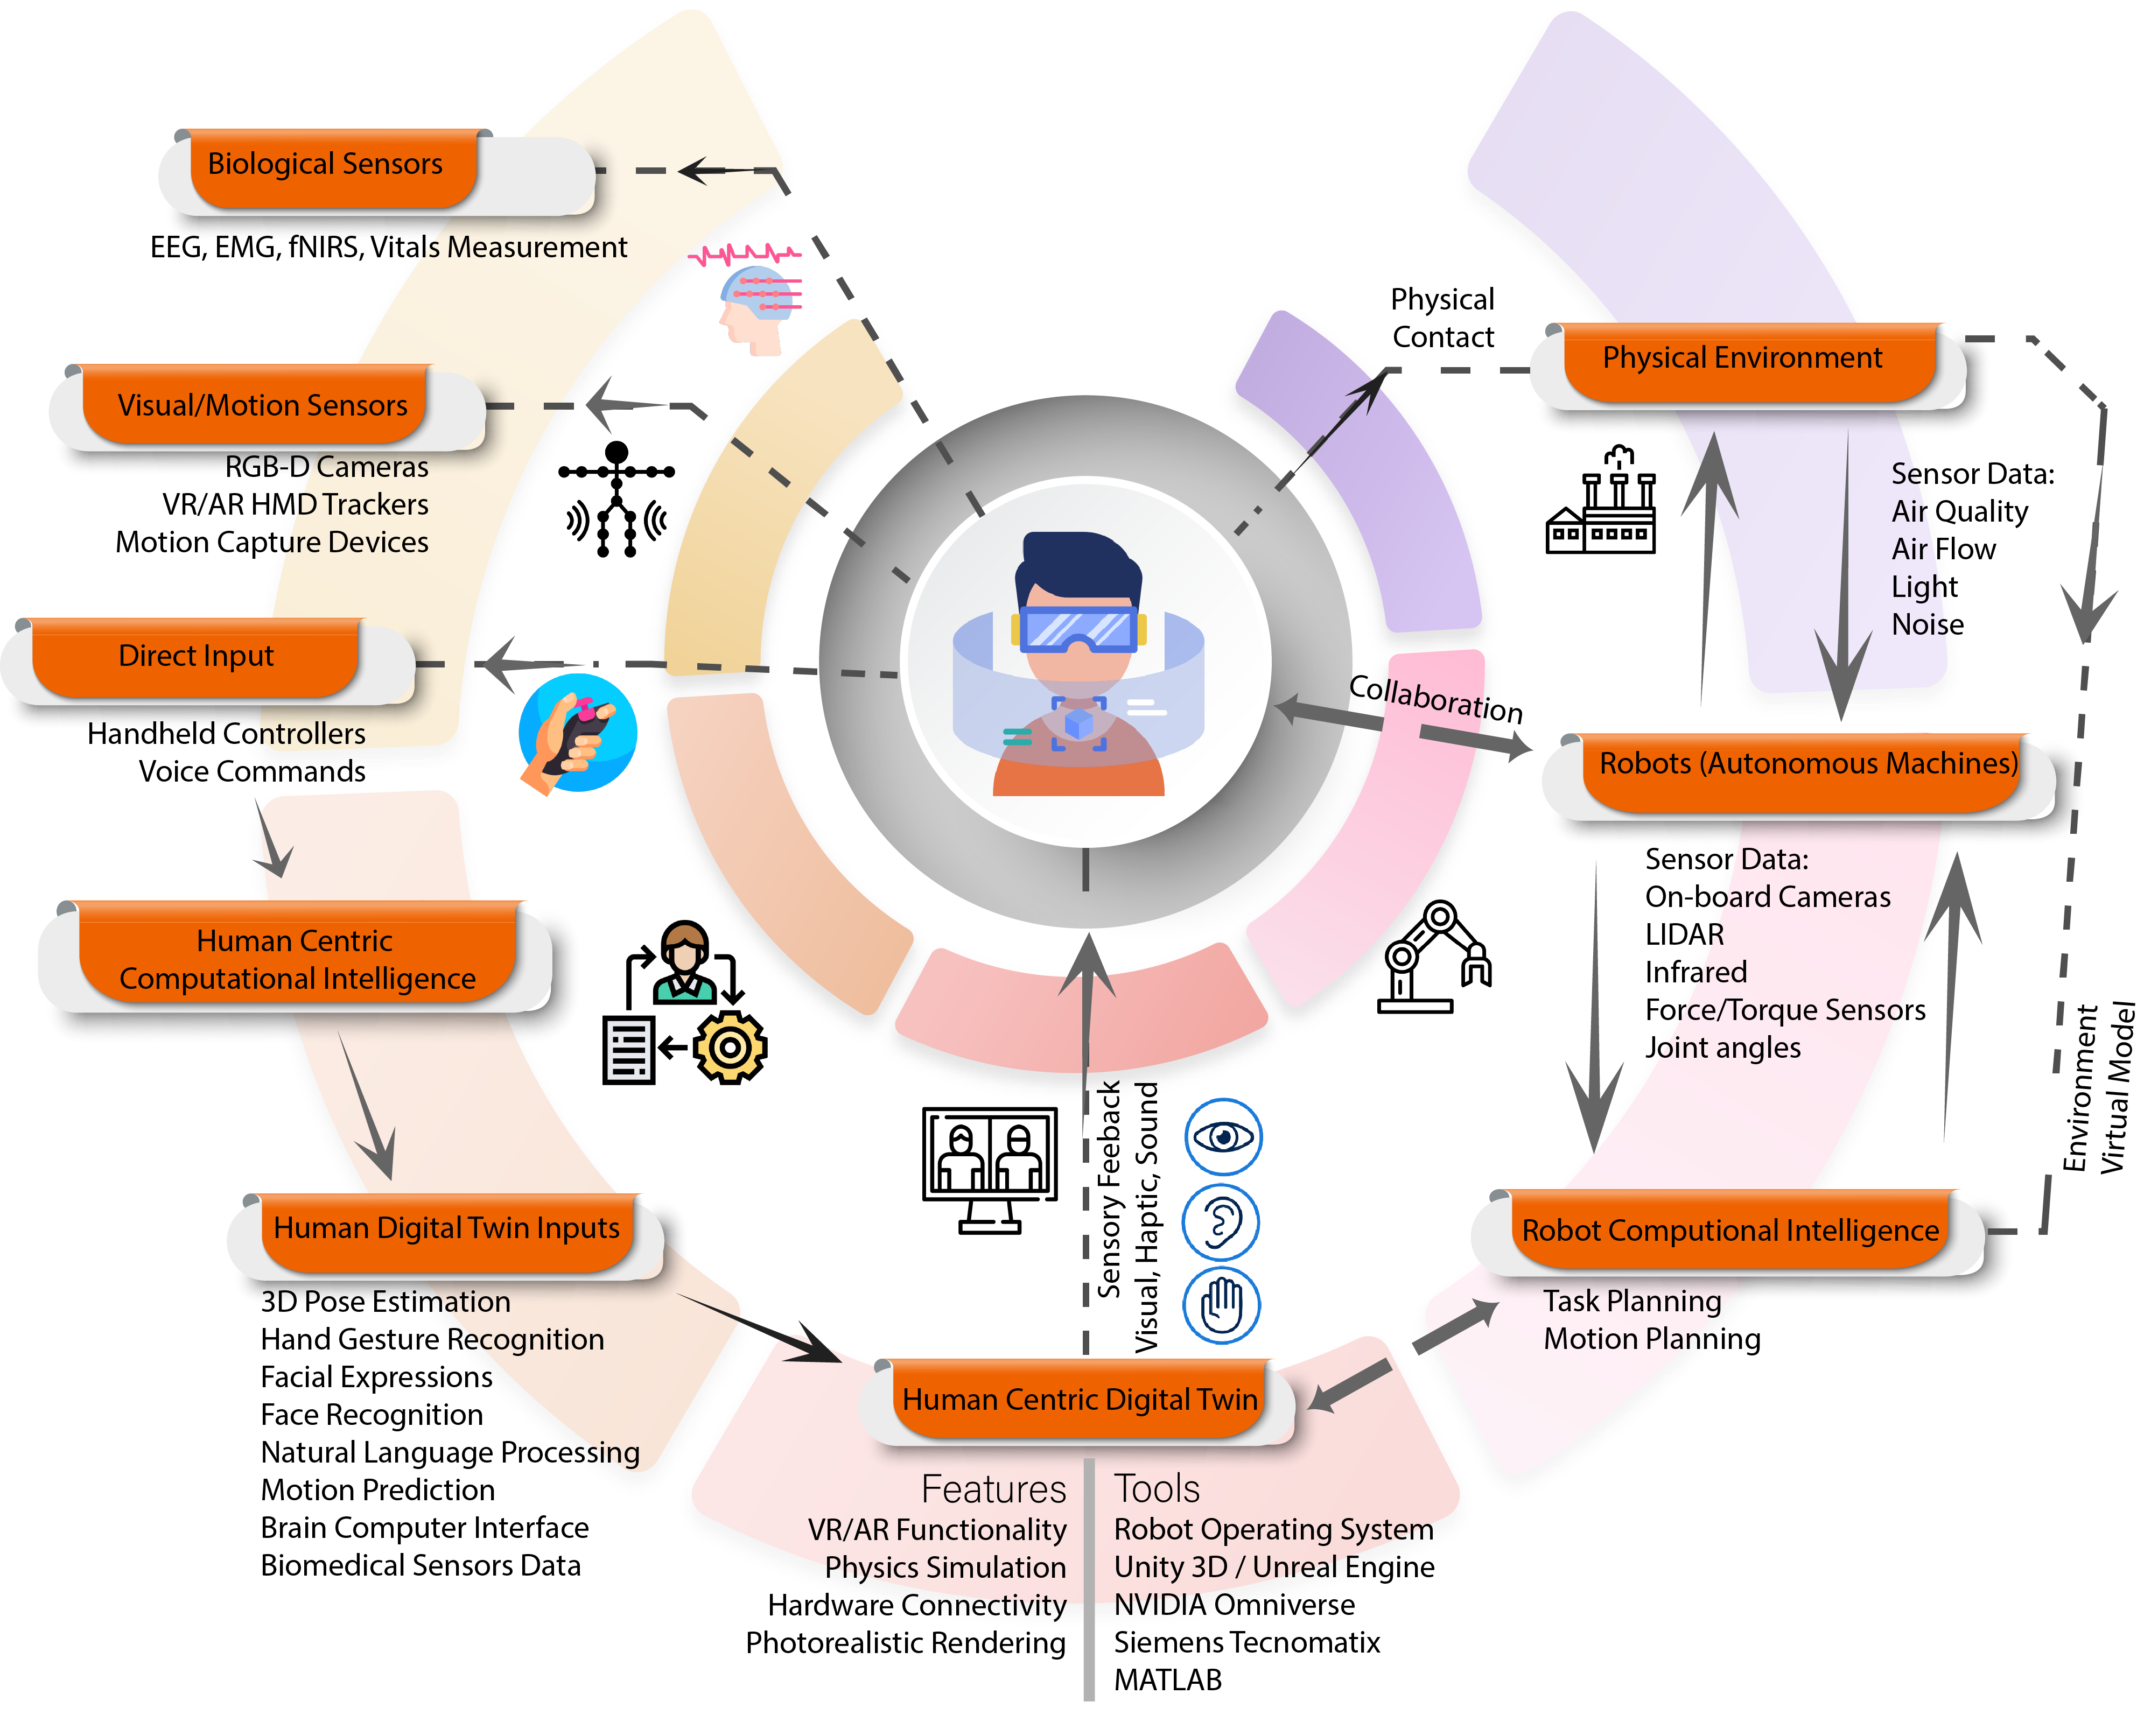
\includegraphics[width=1\linewidth]{ThesisFigs/Framework.png}
    \caption{Enabling Technologies and framework of Human-Centric Digital Twins in Industry 5.0}
    \label{figure:framework1}
\end{figure}

\subsection{Human-focused Sensors}
To create HCDT-driven CPS, sensors are deployed to collect digital data from humans. For accurate human skeletal tracking and joint monitoring, optical and non-optical sensing devices are used. Optical marker-based devices, such as Optitrack and VICON are widely used. On the other hand, optical marker-less technology and video-based human motion tracking devices including RGB-D Cameras \cite{Yi2022, Dimitropoulos2021} and Kinect \cite{Khatib2021, Liu2021} are also extensively used. Non-optical tracking devices include wearable inertial measurement units (IMUs) \cite{Yi2021}.

Different Biological sensors are also being used to measure the physiological data of humans to monitor human behavior during human-robot collaboration \cite{bs1-Tiberio}. Physiological sensors, such as Electroencephalogram (EEG) \cite{bs4-bi} and EMG \cite{bs6-yeom}, capture signals generated from the human body and can infer important information, such as the intention of human operators \cite{bs5-hakonen}.

\subsection{Computational Intelligence}
Artificial Intelligence and Machine Learning are central to realizing the promise of HCDTs.

\subsubsection{Computer Vision}
Creating a high-fidelity Human Digital Twin may involve recognition of human facial features, expression, pose, and gestures. Deep Neural Networks and Computer Vision are being used extensively for this purpose. Yi et al. \cite{Yi2022} uses RGB-D Sensors for posture estimation using a Convolutional Neural Network (CNN). Machine Learning based computer vision has been widely used in literature for safe Human-Robot Collaboration \cite{Droder2018, Osama2019}.

\subsubsection{Classification Methods}
Supervised Learning based classification techniques such as CNNs, Long Short-term Memory (LSTMs), and Hidden Markov Models (HMM) have been used for motion and intent detection and prediction in HRC \cite{Zhang2022-Fusion, AI-MP-Manu, AI-DT-Survey}.

\subsubsection{Reinforcement Learning}
In Reinforcement Learning (RL) algorithms, agents learn their control policy through unsupervised learning. Deep Reinforcement techniques leverage deep neural networks in combination with RL algorithms, such as Q-Learning to solve complex problems. Reinforcement learning has found widespread use in motion planning \cite{Liu2022, Vrabic2021}, and in decision-making in human-centric applications \cite{Sun2022, Xia2021, Matulis2021}.

\subsection{Simulation Tools}
For the development of a DT, different simulation tools are required to create an interaction between physical objects and their virtual twins.

\subsubsection{Numerical Analysis Tools}
Finite Element Analysis (FEA) is often necessary for Multiphysics simulations of physical assets. FEA tools, such as ANSYS \cite{Aubert2021}, COMSOL \cite{Zhu2022} and ABAQUS \cite{Liang2018}, have been frequently used to create DTs for biomedical applications and physical assets for which health/condition monitoring is desired \cite{Aivaliotis2019}.

\subsubsection{Robotics Simulation Tools}
Robotics simulators allow developers to design, test, and evaluate robotic systems in virtual environments. Gazebo is one of the most commonly used simulators \cite{Thumm2022, Bansal2019, Vrabic2021}. It is an open-source simulator that can be integrated with the Robot Operating System (ROS), one of the most widely used platforms by robotics researchers \cite{Macenski2022}.

\subsubsection{Game Physics Engines}
Game development applications and Physics engines are valuable tools for the development and simulation of DTs \cite{Clausen2022}. The most commonly used physics engine is NVIDIA's PhysX, which is used by Unity and Unreal Engine. In recent years, these have widely been used in the development of DTs \cite{BioMech-Eval, Mania2020, Yun2022, Mourtzis2022-MR}.

\subsection{Data Visualization and Interaction}
\subsubsection{Photorealistic Rendering}
The creation of virtual models in DTs begins with 3D modeling tools like Blender \cite{Alexopoulos2020} or 3ds Max \cite{Wu2019}. The ability of these tools to create photorealistic rendered images can be used to generate training data for ML algorithms and to provide a realistic user experience. Often, models are exported to platforms such as NVIDIA Omniverse \cite{Akar2022}, Unity \cite{Dianatfar2021} or Unreal Engine \cite{Mania2020}.

\subsubsection{Immersive User Experience}
The use of DTs creates opportunities for a rich immersive user experience through Virtual Reality, Augmented Reality, and Mixed Reality. In Augmented Reality, virtual objects are superimposed on real images, using a Head Mounted Display (HMD) such as Microsoft Hololens \cite{Kunz2022, Li2022}. Mixed Reality (MR) allows for co-existence and interactivity between the physical and the virtual environment \cite{Ke2019}, which can be used for intuitive teleoperation of robotic manipulators \cite{Su2022}.

\section{Challenges in Deformable Object Manipulation}
Manipulation of deformable materials is a good example of Moravec’s paradox, which states that what is easy for humans tends to be challenging for robots. Human workers frequently perform such manipulation tasks in maintenance, assembly, and manufacturing settings, handling a variety of materials including flexible hoses, cables, textiles, and composite reinforcements. Collaborative robotics and automation have faced persistent challenges in adopting these tasks due to the high dimensionality of deformable materials, which complicates the extraction and representation of their state. Furthermore, there exists a significant sim-to-real gap caused by the challenge of creating high-fidelity simulation and learning environments.

\subsection{Deformable Object Modeling}
Physics-based simulation of deformable materials often relies on geometric representations using particles or meshes. For a thorough review of the foundational aspects of models and dynamics of deformable materials, see \cite{ModelDeformReview}. One of the most promising methods is Position Based Dynamics (PBD) \cite{PBD}. In PBD, objects are represented by a set of vertices and constraints. The simulation predicts new positions for the vertices and then adjusts these positions through an iterative solver to satisfy the constraints. This approach is computationally efficient and robust, making it suitable for real-time applications.

\subsection{Differentiable Simulation and Learning}
Differentiable physics engines have revolutionized robotic manipulation by enabling gradient-based optimization of complex interactions. \cite{Li2023} and \cite{Lin2022} demonstrated how differentiable simulation accelerates skill acquisition for deformable objects. \cite{Liu2023} extended this to cloth manipulation, coupling articulated rigid bodies with deformable models. Complementary to simulation, \cite{Chi2022} introduced iterative residual policies for goal-conditioned manipulation, while \cite{Salhotra2022} leveraged imitation learning to transfer human expertise to robots. These approaches highlight the synergy between simulation fidelity and data-driven learning.

\section{Application Domains}
Digital Twin Technology has recently been applied in a range of industries. Here, we emphasize key application domains where human-centricity is of paramount importance.

\subsection{Ergonomics and Safety}
In Smart Factories, as humans and collaborative robots begin to share workspaces, it is necessary to ensure human safety and optimize ergonomics. Havard et al. \cite{Havard2019} created a DT to carry out a Safety and Ergonomics assessment in VR. In HRC safety, collision avoidance is an important challenge. Liu et al. \cite{Liu2021} employs a deep reinforcement learning algorithm to allow a Cobot to reach a target state while minimizing the risk of collision with a human hand. A generic layout for HCDTs for ergonomics and safety is shown in Figure \ref{figure:FrameworkSafety}.

\begin{figure}[h]
    \centering
    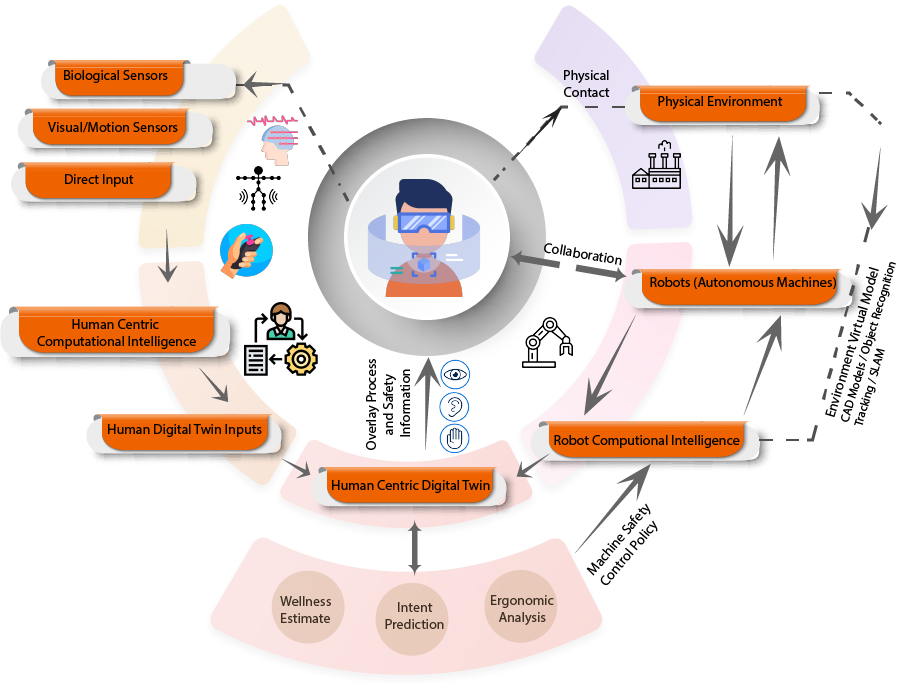
\includegraphics[width=1\linewidth]{ThesisFigs/FrameworkSafety.png}
    \caption{Generic framework for HCDT for safety and ergonomics}
    \label{figure:FrameworkSafety}
\end{figure}

\subsection{Training and Testing of Robotics Systems}
DTs have found great utility in the training and testing of Robotics Systems. DTs can provide a high-fidelity virtual environment to generate a vast amount of test data to viably train an ML model and transfer it to the physical robot. NVIDIA has demonstrated this capability using its platform NVIDIA Omniverse to create DTs of warehouses for training of AI models \cite{omniverse}. Mania et al. employed photorealistic simulations rendered in a game engine to increase the performance of the perception system of a mobile robot \cite{Mania2020}. A generic framework for using HCDTs for training robotics systems is shown in Figure \ref{figure:FrameworkML}.

\begin{figure}[h]
    \centering
    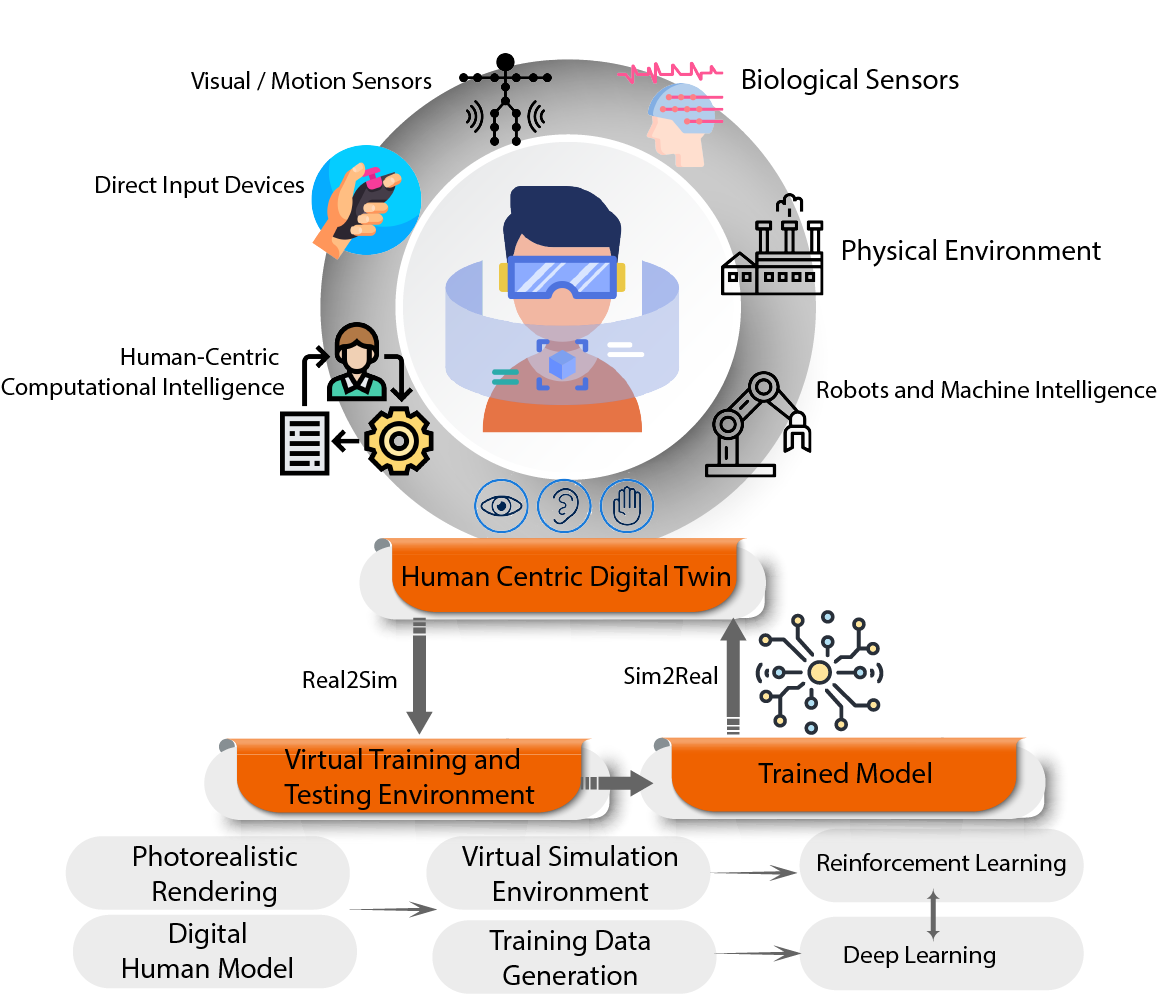
\includegraphics[width=1\linewidth]{ThesisFigs/TrainingFrameworkReduced2.png}
    \caption{Generic framework for Robotics System Training}
    \label{figure:FrameworkML}
\end{figure}

\subsection{User Training and Education}
VR/AR technologies are already widely used in training and teaching. The use of AR/VR headsets enable operators to get a better understanding of a process, for remote assistance and operator training \cite{Perno2022}. DTs have also been used in enhanced surgical training, where the use of DTs with haptic feedback is reported to increase accuracy and reduce cognitive load on surgeons \cite{Hagmann2021}.

\subsection{Product and Process Design, Validation and Testing}
The prospect of using DTs in combination with immersive technologies can be utilized to enhance and enrich the process and product design. Malik et al. \cite{Malik2019-Tariq} leveraged DTs and virtual reality for HRC design and planning. The proposed architecture uses bi-directional information sharing between the physical and virtual robot and human operator. In the VR environment, designers can manipulate objects and study the HRC design from the perspective of visibility, reach, and ergonomics to optimize cycle times and safety.

\subsection{Security of Cyber-Physical systems}
Security and reliability are important issues in DTs, more so in HCDTs. In the context of a Collaborative Robotic Cyber-Physical System (CRCPS), Khalid et al. present a framework for secure CRCPS based on authentication and data integrity checks \cite{Khalid2018}. Digital Twins can themselves be used for enhancing security: Deitz et al. sets out formal requirements of a security framework that employs DT simulations to detect, analyze and handle security incidents \cite{Dietz2020}.

\subsection{Rehabilitation, Well-being and Health Management}
In the medical domain, Human Digital Twin technology has found more maturity and acceptance. Medical Digital Twins (MDTs) have been used in many areas including pulmonology \cite{Zhang2021} and orthopedics \cite{Hernigou2021}. MDTs may involve using clinical imaging techniques to develop Patient-specific solutions, for example for the human tongue \cite{Calka2021}, tibia \cite{Aubert2021}, or aortic walls \cite{Liang2018}. Figure \ref{figure:MedicalFramework} illustrates a generic layout for healthcare applications.

\begin{figure}[h]
    \centering
    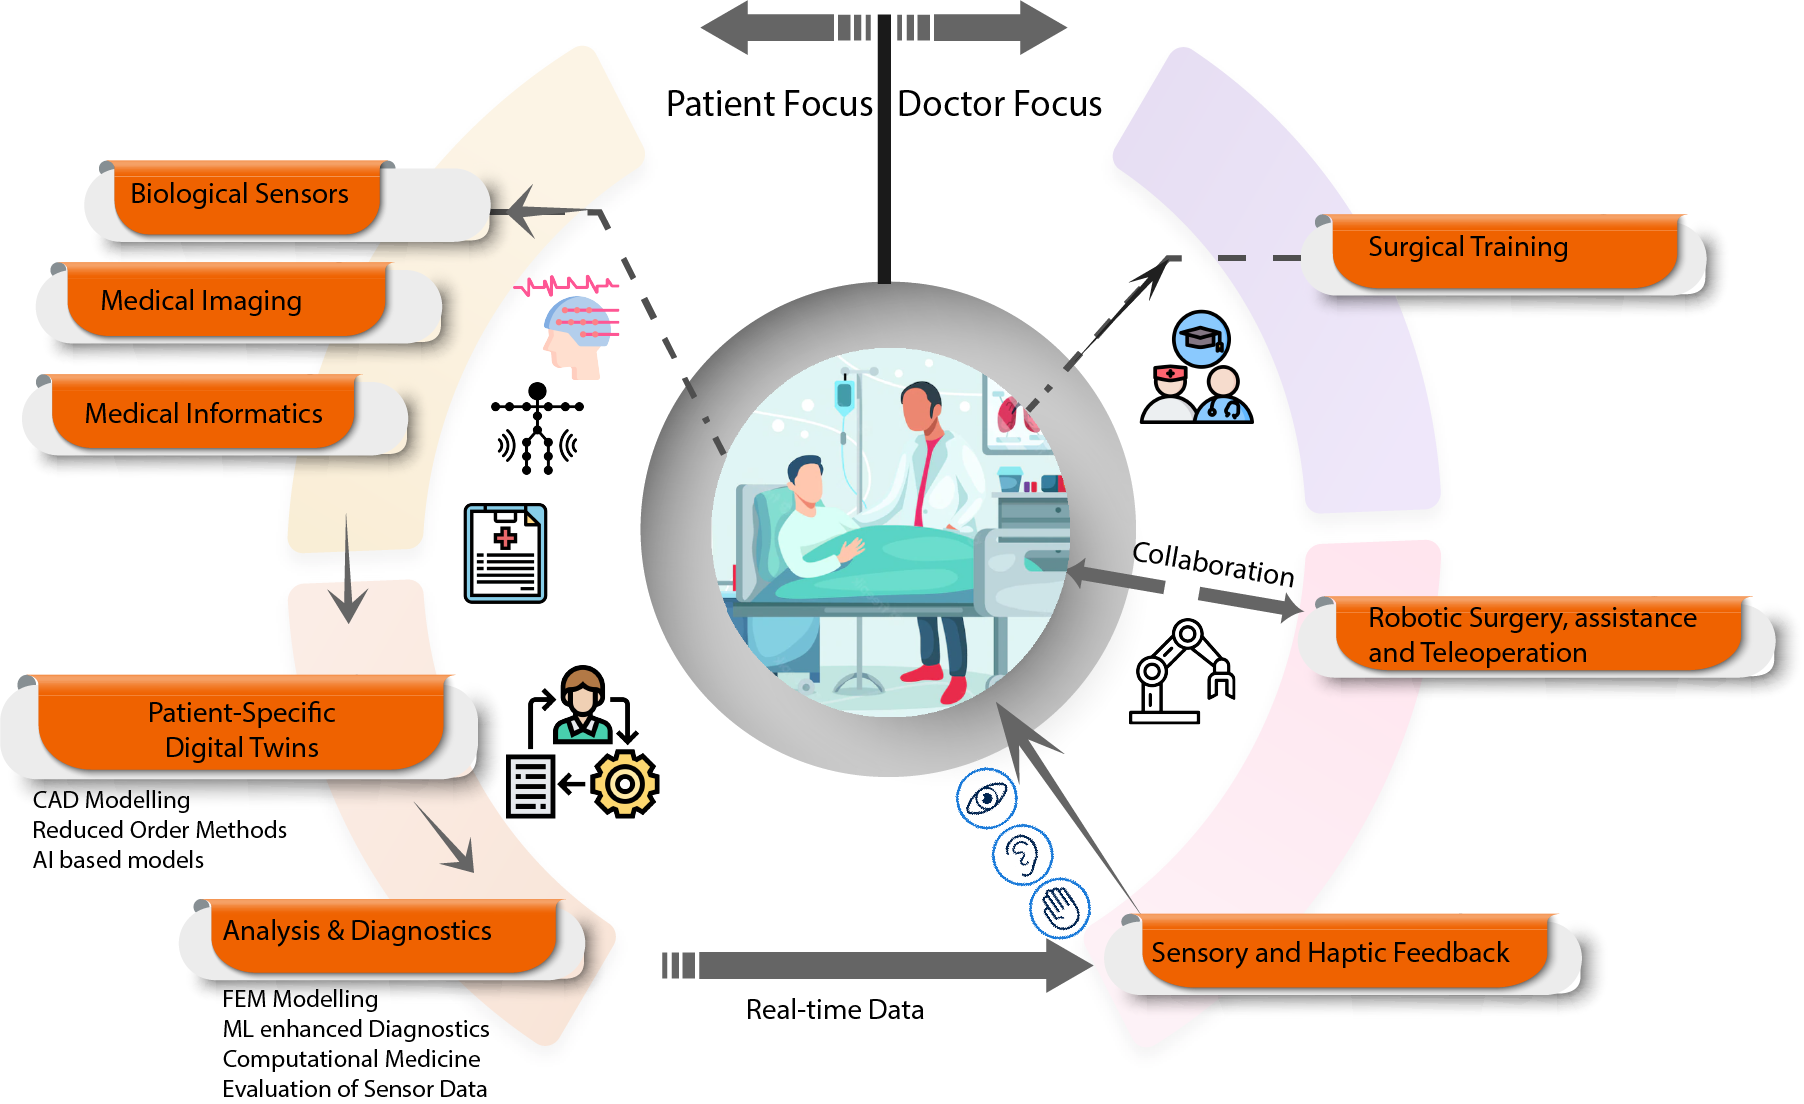
\includegraphics[width=0.9\linewidth]{ThesisFigs/MedicalFramework.png}
    \caption{Generic framework for DTs in healthcare}
    \label{figure:MedicalFramework}
\end{figure}

\section{Research Gap}
This chapter has provided a comprehensive review of Human-Centric Digital Twins, their enabling technologies, and key application domains. A key shortcoming observed from current DT literature is that the focus is almost entirely on the physical assets of a CPS, and not on human operators. To address this, a deeper understanding of human intent and motion is required, especially for complex tasks such as the manipulation of deformable objects. The enabling technologies for this purpose, such as AI-driven algorithms for object recognition and collision avoidance, have reached some degree of maturity. However, there is a lack of literature in which all these enabling technologies are utilized together in a synergistic manner to enhance human-machine interaction in industrial settings. The following chapters will detail a novel framework designed to bridge this gap, with a specific focus on developing proactive robotic assistance for composites manufacturing.
 % Background Theory
\clearpage
\lhead{\emph{Human Intention and Motion Prediction Framework}}  % Set the left side page header to "Contents"
\chapter{Human Intention and Motion Prediction Framework}
\label{chap:framework}

%----------------------------------------------------------------------------------------
\section{Introduction}
%----------------------------------------------------------------------------------------

The paradigm of Digital Twins has found widespread application in optimizing performance across diverse industrial sectors, including manufacturing, aerospace, and energy \citep{Andronas2021, Polini2020}. However, conventional digital twins often prioritize technical system aspects, frequently overlooking the human element crucial for Industry 5.0. Human-Centric Digital Twins (HCDTs) aim to address this by integrating models of human behavior, cognition, and even emotion, thereby enabling personalized and adaptive feedback to human operators \citep{Usman}. A truly effective HCDT allows the predicted intention and motion to be utilized in several ways: for real-time monitoring of operator performance, for providing semantic assistance, such as prompting the operator on the next step or flagging procedural errors, and for enabling a robotic assistant to proactively provide physical support.

Such HCDTs promise to elevate safety, efficiency, and productivity in human-machine systems, while concurrently enhancing user experience and satisfaction \citep{Umbrico2022}. In high-mix, low-volume (HMLV) industrial contexts, traditional automation systems exhibit significant rigidity, necessitating substantial human intervention for customization and adaptation. The advent of Machine Learning (ML), Artificial Intelligence (AI), and advanced automation technologies offers a pathway towards more flexible solutions, particularly beneficial for Small and Medium Enterprises (SMEs). These innovations can facilitate partial automation of labor-intensive tasks or enable collaborative human-robot workflows, where humans focus on complex reasoning and dexterous manipulation, while robots manage repetitive actions \citep{Cotta2023, Sirintuna2024}.

Current AI systems are approaching a semantic understanding of human actions and intentions, but translating this understanding into accurate 3D motion prediction remains an open problem. This predictive capability is paramount for robots to transition from reactive assistance to smart collaboration. To address this challenge, this chapter presents a modular and scalable framework that utilizes Vision-Language Models (VLMs) with motion diffusion techniques to predict human intent and generate plausible future human motion in semi-structured environments.

\subsection{Motivation for a Modular Approach}

Instead of pursuing end-to-end training, the approach presented in this thesis emphasizes the integration of existing, pre-trained perception and reasoning modules. This design philosophy not only makes the system more practical for SMEs with limited computational resources and training data, who can benefit from leveraging pre-trained foundation models rather than training custom models from scratch, but also ensures adaptability, as overall framework performance can improve with advancements in individual modules without requiring complete system re-training. The modular design further allows for inspection and debugging of intermediate outputs, facilitating understanding of system behavior and failure modes, and different modules can be swapped or upgraded independently based on application requirements or available computational resources.

This modular philosophy directly addresses the limitations identified in Chapter~\ref{chap:literature}, where existing approaches either focus narrowly on action recognition within limited classes or produce context-agnostic pose forecasts that fail to account for task semantics and environmental constraints.

\subsection{Chapter Overview}

The remainder of this chapter is organized as follows. Section~\ref{sec:framework_architecture} presents the high-level architecture of the proposed framework, introducing its three primary modules and their interconnections. Section~\ref{sec:perception_scene} details the Perception and Scene Representation module, covering human pose estimation, 3D scene grounding, and gaze analysis. Section~\ref{sec:ai_reasoning} describes the AI-Driven Reasoning and Intent Prediction module, including task knowledge representation and the two-phase prediction pipeline. Section~\ref{sec:motion_generation} presents the Human Motion Generation module, which synthesizes physically plausible 3D motion from predicted intent. Finally, Section~\ref{sec:chapter_summary} summarizes the key contributions of the proposed framework.

%----------------------------------------------------------------------------------------
\section{Proposed Framework Architecture}
\label{sec:framework_architecture}
%----------------------------------------------------------------------------------------

A modular framework is proposed to enable intelligent Human-Robot Collaboration (HRC) by predicting human intention and future pose. This methodology is designed to bridge the gap between short-term motion forecasting and long-term action planning, ensuring predictions are both physically plausible and contextually appropriate.

\subsection{High-Level Overview}

Formally, the predictive challenge is to process a stream of multimodal data to predict human intention and motion. Let the input at any given time $t$ consist of a history of video frames $\mathcal{V} = \{I_k\}_{k=1}^t$, extracted human poses $\mathcal{P} = \{P_k\}_{k=1}^t$, and static, high-level task knowledge $\mathcal{C}_{task}$. The framework, represented by a function $\mathcal{F}$, processes this context to give three outputs: the predicted task state $S_t$, which captures the current progress within the overall workflow; a forecast of future hand positions $\hat{H}_{t+\Delta t} = ( (x_l, y_l), (x_r, y_r) )$, for a time horizon $\Delta t$; and a full-body 3D motion trajectory $\hat{M}_{t_i} = \{\hat{x}_{t_i+1}, \ldots, \hat{x}_{t_i+N_{\text{pred}}}\}$.

The proposed framework, illustrated in Figure~\ref{fig:framework_overview}, has three primary modules that work in concert to achieve context-aware motion prediction.

\begin{figure}[htbp]
    \centering
    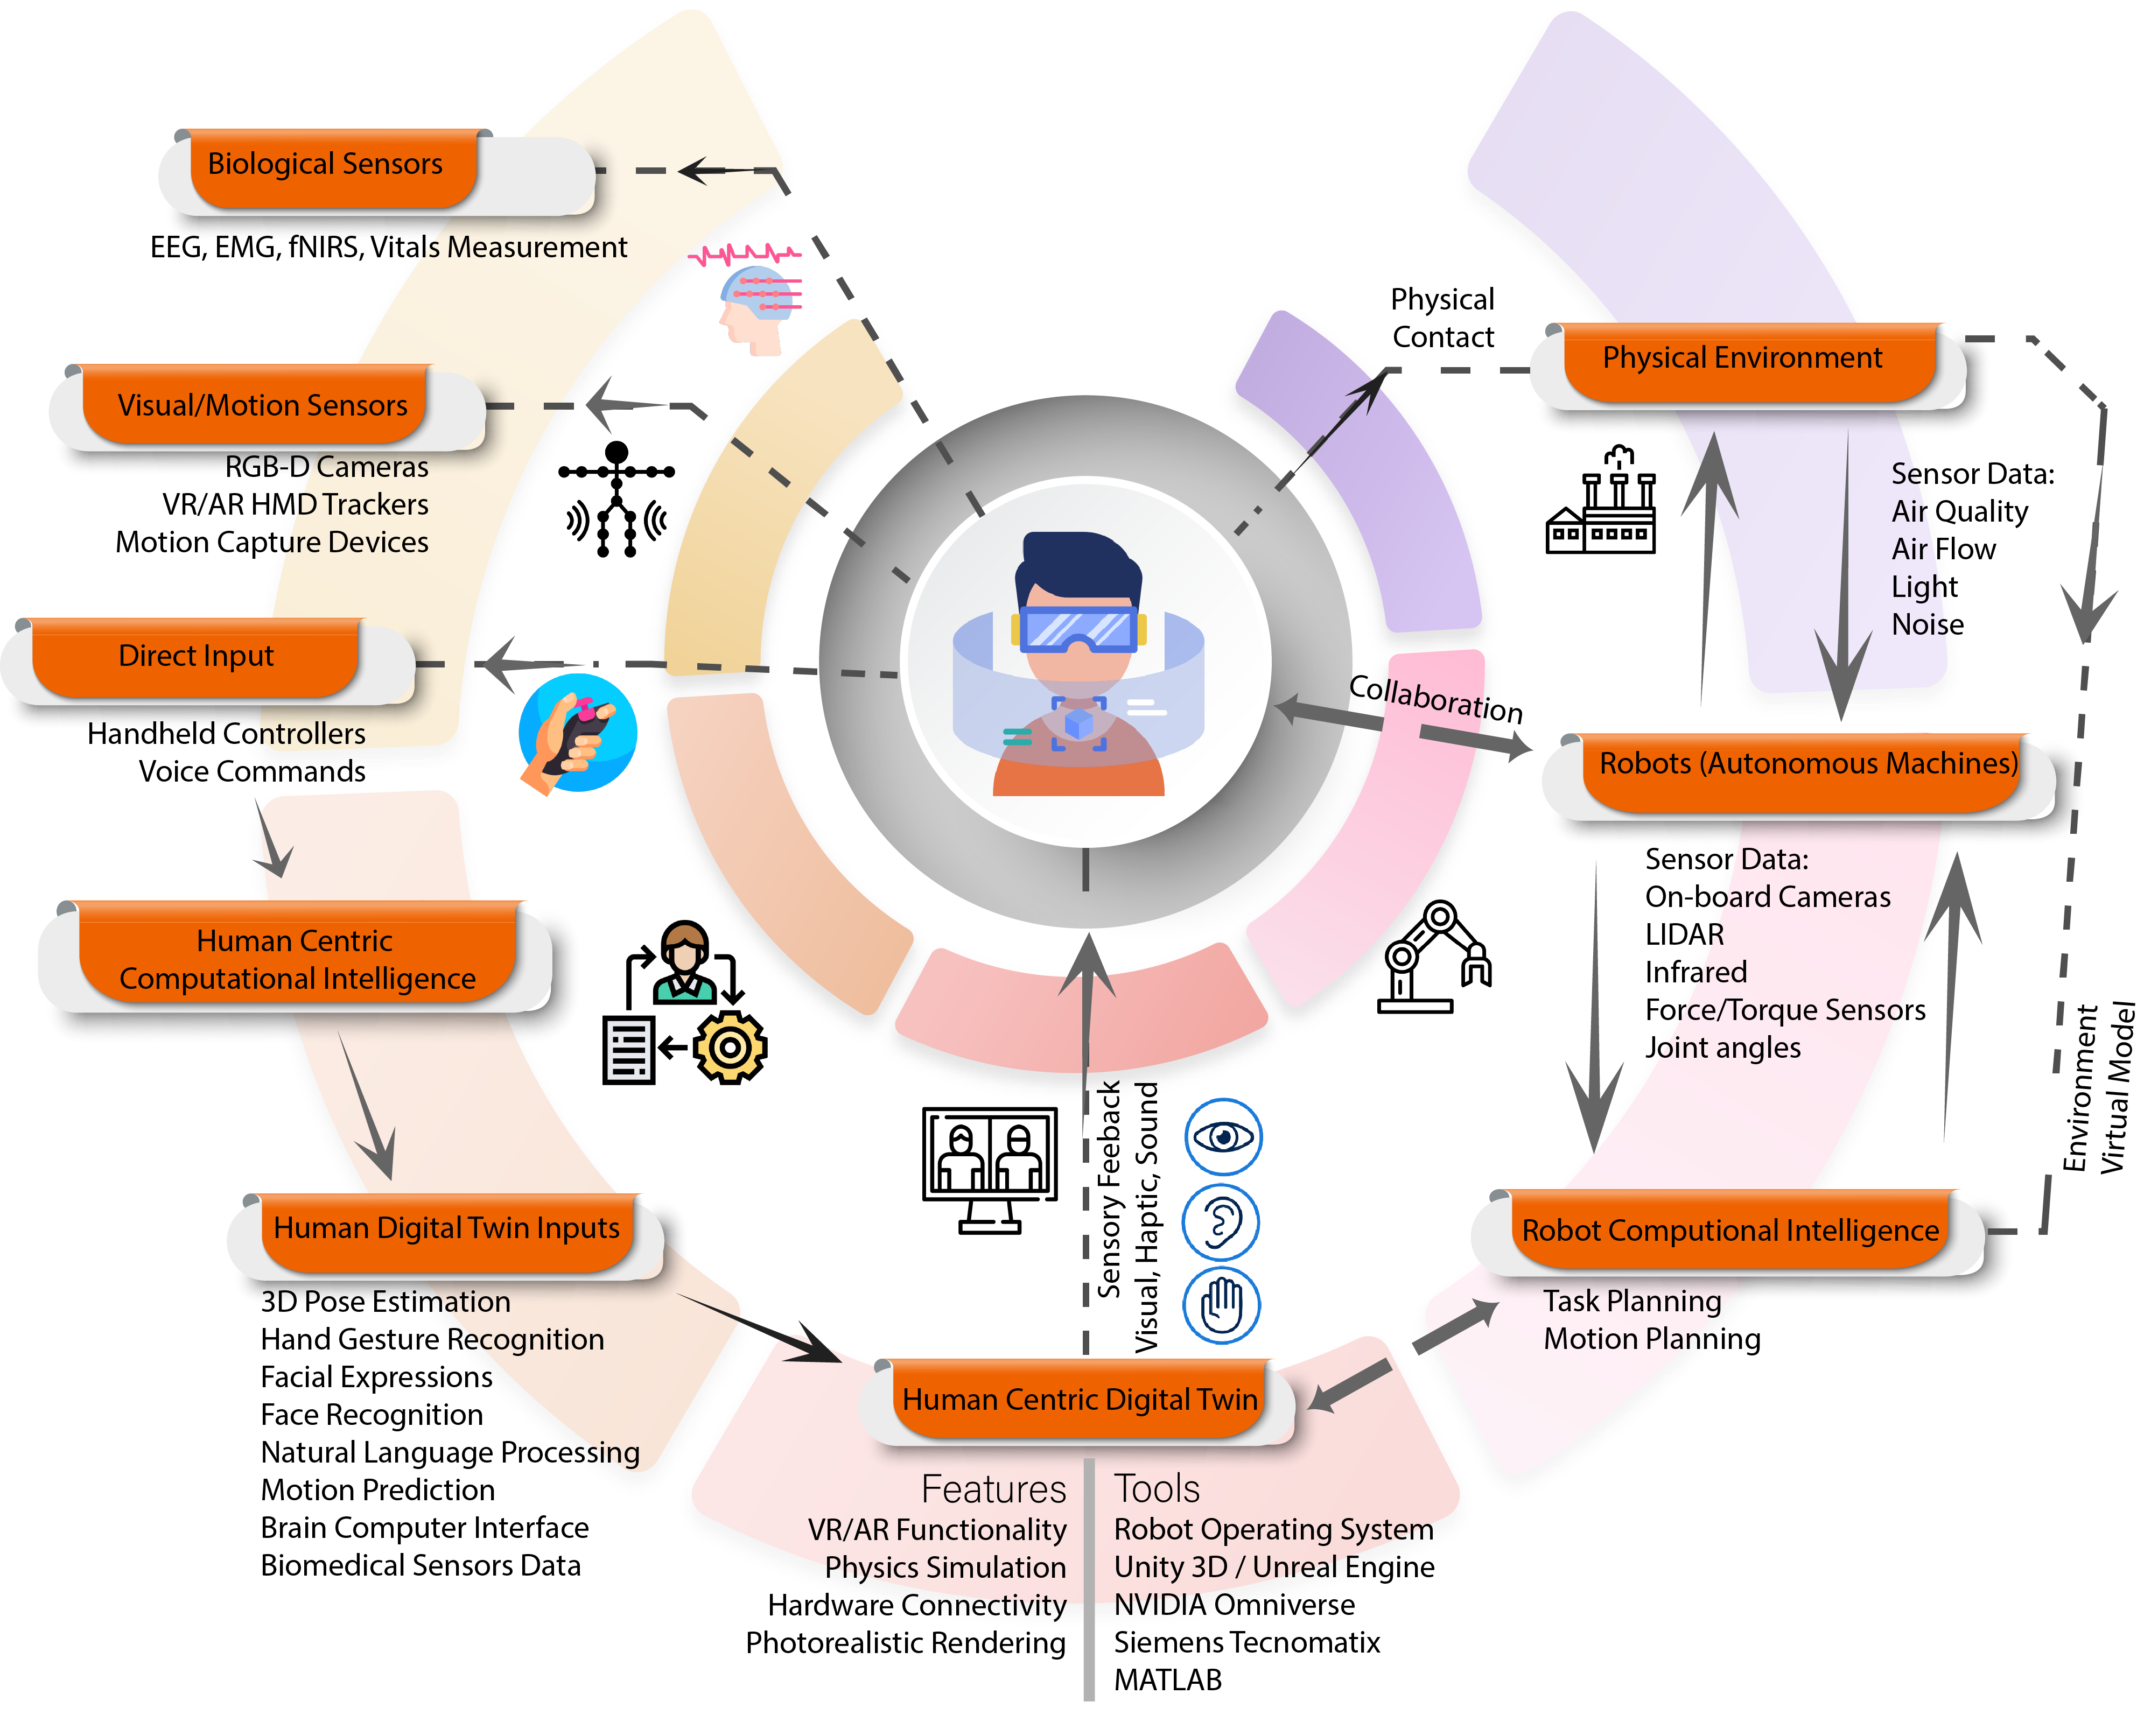
\includegraphics[width=\textwidth]{ThesisFigs/Framework.png}
    \caption{Conceptual overview of the proposed modular framework for Human Intention Prediction based Motion Generation. Information flows from the physical system through the perception and reasoning modules to generate a final motion prediction.}
    \label{fig:framework_overview}
\end{figure}

\subsubsection{Perception and Scene Representation Module}

The Perception and Scene Representation Module serves as the sensory foundation of the framework. It processes raw visual data from cameras to extract meaningful representations of the human operator and the surrounding environment. Key functions include extracting human pose parameters using state-of-the-art human mesh recovery techniques, estimating metric depth to enable 3D scene understanding, tracking human gaze targets to provide cues about operator attention and intent, and converting 2D visual predictions into world-frame 3D coordinates.

\subsubsection{AI-Driven Reasoning and Intent Prediction Module}

The AI-Driven Reasoning and Intent Prediction Module serves as the cognitive core of the framework. It leverages Vision-Language Models (VLMs) to interpret the current task context based on structured task knowledge, predict the current task state and progress within the workflow, forecast future hand positions based on inferred intent, and generate semantic understanding of operator actions and goals. This module bridges the gap between low-level perceptual data and high-level semantic understanding, enabling the system to reason about what the operator is trying to accomplish rather than simply tracking their current pose.

\subsubsection{Human Motion Generation Module}

The Human Motion Generation Module transforms the high-level predictions from the reasoning module into full-body 3D motion trajectories. It employs diffusion-based motion synthesis conditioned on predicted intent, physics-based refinement to ensure motion plausibility, and integration with digital twin visualization for operator feedback. This modularity allows for individual modules to be upgraded as technology advances. While the framework provides the necessary predictive outputs for a complete Human-Centric Digital Twin (HCDT), the implementation of feedback and physical assistance mechanisms is designated as future work.

%----------------------------------------------------------------------------------------
\section{Perception and Scene Representation}
\label{sec:perception_scene}
%----------------------------------------------------------------------------------------

The Perception and Scene Representation module is responsible for extracting structured information from raw visual inputs. This section details the specific techniques employed for human pose estimation, 3D scene understanding, and gaze analysis.

\subsection{Human Pose Representation}

Accurate and expressive human pose representation is fundamental to the framework's ability to understand and predict human motion. This subsection describes the hierarchical approach to pose representation, from the underlying parametric model to the kinematic format used for motion generation.

\subsubsection{SMPL-X Model for Whole-Body Representation}

The framework adopts the Skinned Multi-Person Linear Model with Extensions (SMPL-X) \citep{SMPL-X:2019}, which provides a parametric model for body shape $\boldsymbol{\beta}$, pose $\boldsymbol{\theta}$, and expressive hand and face parameters $\boldsymbol{\psi}$. The SMPL-X model generates a mesh $M(\boldsymbol{\beta}, \boldsymbol{\theta}, \boldsymbol{\psi})$ through a learned blend shape function, enabling realistic representation of human body configurations. The model's differentiable nature allows for gradient-based optimization when fitting to visual observations.

\subsubsection{Global-View Human Mesh Recovery (GVHMR)}

To obtain the pose parameters from monocular RGB video, the framework employs World-Grounded Human Motion Recovery via Gravity-View Coordinates (GVHMR) \citep{multi-hmr2024, gvhmr}. GVHMR reconstructs human pose in a global, gravity-aligned coordinate system, which is essential for the framework as it provides consistent spatial reference across frames, facilitates integration with 3D scene understanding by placing both human and environment in the same coordinate frame, and enables physics-based motion refinement by providing ground-plane alignment. GVHMR outputs the transformation between global and camera coordinates $(R_{wc}, \mathbf{t}_{wc})$, which is used for subsequent 3D scene grounding operations.

\subsubsection{Kinematic Representation for Motion Generation (HumanML3D)}

For kinematic motion generation, the SMPL-X poses are subsequently converted into the representation utilized by HumanML3D \citep{Guo_2022_CVPR}. This format captures frame-relative information such as root angular and linear velocities ($\dot{r}_a, \dot{r}_x, \dot{r}_z$), root height ($r_y$), and local joint positions, rotations, and velocities ($j_p, j_r, j_v$), along with foot contact features ($f$). This relative encoding facilitates the generation of smooth and continuous motions by capturing the dynamics of movement rather than absolute positions.

\subsection{3D Scene Grounding and Contextual Cues}

Beyond human pose estimation, the framework requires understanding of the 3D environment and the operator's attention patterns. This subsection describes the techniques for metric depth estimation and gaze analysis.

\subsubsection{Metric Depth Estimation and World-Frame Conversion}

The module converts the VLM's 2D predictions into 3D world coordinates by combining world-frame human pose reconstruction results and metric depth estimation. Modern monocular depth estimation models, such as Unik3D \citep{unik3d}, provide metric-scale depth predictions from single images.

By leveraging the global-to-camera transformation $(R_{wc}, \mathbf{t}_{wc})$ provided by GVHMR, camera-centric 3D points $\mathbf{x}_c$ can be transformed into a consistent world frame via:
\begin{equation}
    \mathbf{x}_w = R_{wc}^\top (\mathbf{x}_c - \mathbf{t}_{wc})
\end{equation}

This transformation allows any point of interest (POI), such as a tool or a predicted hand location, to be localized in the global reference frame. For specialized applications requiring different or higher-precision grounding, this module can be extended to incorporate other engineered approaches, such as processing fiducial markers or leveraging structured light sensors.

\subsubsection{Human Gaze Target Analysis for Intent Inference}

Human gaze provides a strong cue for immediate intent. Research in cognitive science has established that gaze typically precedes manual action by several hundred milliseconds, making it a valuable predictive signal. A change in the operator's gaze target serves as an indicator of a change in intention, and the location of the gaze target often correlates with the area or object the operator intends to interact with next. Techniques like Gaze-LLE \citep{ryan2024gazelle} can be employed for gaze target tracking to further enrich the context provided to the reasoning and intent prediction module.

%----------------------------------------------------------------------------------------
\section{AI-Driven Reasoning and Intent Prediction}
\label{sec:ai_reasoning}
%----------------------------------------------------------------------------------------

This module serves as the cognitive core of the framework, responsible for interpreting the perceptual data within the context of structured task knowledge and generating predictions about operator intent and future actions.

\subsection{Task Knowledge Representation}

The integration of VLMs for high-level reasoning about tasks and intent requires appropriate data structures to represent task knowledge. This subsection describes the formalisms used and the process for generating task context.

\subsubsection{Directed Acyclic Graphs (DAGs) for Procedural Tasks}

Task dependencies are modeled using formalisms like Directed Acyclic Graphs (DAGs), which define the valid sequence of actions and states within a workflow. Alternative formalisms, such as Planning Domain Definition Language (PDDL) \citep{Singh2023}, Knowledge Graphs (KGs), or Behavior Trees (BTs) \citep{Ahn2022, IEEE-Knowledgebased2021}, can also be integrated depending on application requirements.

\subsubsection{AI-Assisted Generation of Task Context}

For any use case, a common operational flow is followed for establishing task context. Initially, task-specific knowledge, such as assembly instructions, procedural steps, or an example video, is provided to the system. This involves a collaborative effort where an AI model generates an initial draft of a task representation (i.e., the overall goal, a mechanism for state tracking, decomposition into smaller actions, and their dependencies), which is then refined by human experts. This task representation forms a critical part of the context provided to the VLM for prediction.

\subsection{Two-Phase Prediction Pipeline}

The prediction process follows a two-phase approach that decouples long-horizon semantic reasoning from short-horizon spatiotemporal forecasting. This separation allows each phase to be optimized with the most relevant context.

\subsubsection{Phase 1: Task State Prediction}

In the first phase, the VLM analyzes video frames along with appropriate context from the perception module and the task graph. The output is an updated Task State in a structured JSON format, identifying the steps completed, steps in progress, steps available, and the immediate next step. This phase addresses the question of \emph{what} the operator is doing and \emph{where} they are in the overall workflow.

\subsubsection{Phase 2: Future Hand Position Forecasting}

In the second phase, the VLM uses the updated task context along with multimodal data from the perception module to forecast the exact pixel coordinates $(\texttt{x}, \texttt{y})$ for both of the operator's hands at a future time horizon $\Delta t$. This two-phase approach is crucial because it decouples long-horizon semantic reasoning about the overall task from short-horizon spatiotemporal forecasting of immediate motion, allowing each phase to be optimized with the most relevant context. This two-phase pipeline is illustrated in Figure~\ref{fig:prediction_pipeline}.

\begin{figure}[htbp]
    \centering
    \subfloat[Task State Prediction]{
\includegraphics[width=0.48\textwidth, trim=5 0 235pt 0, clip]{ThesisFigs/s5.png}\label{fig:task_state_prediction}}
    \hfill
    \subfloat[Hand Position Forecasting]{
\includegraphics[width=0.48\textwidth, trim=5 0 235pt 0, clip]{ThesisFigs/s6.png}\label{fig:hand_prediction}}
    \caption{The two-phase pipeline of the Reasoning and Intent Prediction Module: (a) In the first phase, the VLM uses the task graph and visual information to update the overall task state. (b) In the second phase, it uses this state along with a sequence of recent frames and additional context to predict the operator's future hand positions.}
    \label{fig:prediction_pipeline}
\end{figure}

\subsection{VLM Prompting Strategies for Intent Prediction}

The effectiveness of VLM-based prediction depends critically on how context is structured and presented. This subsection describes three prompting strategies investigated for optimizing predictive accuracy.

\subsubsection{Baseline: Single-Image Input}

The simplest approach provides only a single current frame to the VLM along with the task graph and state representation. While computationally efficient, this strategy consistently underperforms due to the lack of historical context or ``memory,'' rendering it unable to distinguish between similar visual states that differ in their history. This baseline is evaluated in Chapter~\ref{chap:validation}.

\subsubsection{Rolling Context Window (RCW) for Temporal Analysis}

The Rolling Context Window (RCW) strategy provides the VLM with a window of recent frames (typically 10 frames spaced at 1-second intervals) along with the predicted state from the previous prediction cycle. This approach offers a balance of performance and efficiency, providing temporal context for observing motion patterns while achieving near real-time predictions (2-3 seconds) with efficient models. However, RCW is susceptible to \emph{consistency bias}: if the model erroneously determines a step to be completed, it often fails to revise this belief, causing subsequent predictions to suffer from error propagation.

\subsubsection{In-Context Learning (ICL) with Full Task Examples}

The In-Context Learning strategy provides the VLM with a complete example video of the task along with its corresponding ground-truth state evolution. While ICL achieves the highest accuracy in controlled experiments, the requirement for a large context token count results in significant computational latency and, in some cases, a paradoxical degradation of predictive accuracy due to ``overthinking'' \citep{inversescaling}, thus rendering the approach unsuitable for real-time applications. The trade-offs between these strategies are analyzed in detail in Chapter~\ref{chap:validation}.

%----------------------------------------------------------------------------------------
\section{Human Motion Generation}
\label{sec:motion_generation}
%----------------------------------------------------------------------------------------

As a final, downstream step, the high-level predictions from the Reasoning and Intent Prediction Module drive the Motion Generation Module. This module is crucial for visualizing the predicted intent as a full-body 3D motion and for providing the basis for robot motion planning in collaborative scenarios.

\subsection{Kinematic Motion Synthesis from Intent}

The core of this module adapts diffusion-based motion synthesis techniques to generate plausible future motion conditioned on the predicted intent.

\subsubsection{Adapting the Motion Diffusion Model (MDM)}

The framework builds upon the Human Motion Diffusion Model (MDM) \citep{tevet2023human} and its physics-aware extension CLoSD \citep{tevet2024closd}. The diffusion process operates as follows:

\textbf{Forward Process:} The forward diffusion process $q(x_t|x_{t-1})$ gradually adds Gaussian noise to a motion sequence:
\begin{equation}
    q(x_t|x_{t-1}) = \mathcal{N}(x_t; \sqrt{\alpha_t}x_{t-1},(1-\alpha_t)I)
\end{equation}

where $\alpha_t$ is a noise schedule parameter.

\textbf{Reverse Process:} The reverse process $p_\theta(x_{t-1}|x_t)$ learns to denoise the motion:
\begin{equation}
    p_\theta(x_{t-1}|x_t) = \mathcal{N}(x_{t-1}; \mu_\theta(x_t,t),\sigma_t^2 I)
\end{equation}

The model is trained to minimize an L2 reconstruction loss:
\begin{equation}
    \mathcal{L}_{\text{simple}} = \mathbb{E}_{x_0,t}[\|x_0 - \hat{x}_0\|_2^2]
\end{equation}

\subsubsection{Conditioning on Predicted Task and Target Locations}

The model receives the previous 40 frames of motion data in HumanML3D format and synthesizes future motion sequences for the next two seconds (60 frames at 30 fps). This is additionally conditioned on a textual prompt describing the predicted action or intent, and a target joint (e.g., \texttt{right\_wrist}, \texttt{pelvis}) with its target 3D location derived from the hand position prediction. The Human Motion Model hence synthesizes a physically plausible and semantically guided future motion sequence.

\subsection{Physics-Based Refinement for Plausibility}

Purely kinematic motion synthesis often produces physically implausible results with artifacts such as foot sliding during locomotion, ground penetration or floating, and unnatural joint velocities or accelerations. The CLoSD framework \citep{tevet2024closd} addresses these issues by closing the loop between motion planning and execution. It uses a real-time, autoregressive Diffusion Planner (DiP) to generate kinematic motion plans on-the-fly, which are then executed by a robust reinforcement learning-based tracking controller in a physics simulator. This approach ensures that the final motion respects physical constraints while remaining faithful to the intended action.

\subsection{Visualization in the Digital Twin Environment}

The generated motion sequences are visualized within a virtual representation of the real environment given by a 3D point cloud created by the perception module's depth estimation model. This visualization serves multiple purposes: operators and system designers can visually verify that predictions are reasonable, the digital twin can be used for operator training or for simulating collaborative scenarios, and the predicted human motion provides input for robot motion planning algorithms to ensure safe and efficient collaboration. Figure~\ref{fig:motion_visualization} illustrates sample motion generation results.

\begin{figure}[htbp]
    \centering
    \subfloat[Ground truth motion]{
\includegraphics[width=0.48\textwidth, trim=0 0 0 40, clip]{ThesisFigs/s3.png}}
    \hfill
    \subfloat[Generated motion]{
\includegraphics[width=0.48\textwidth, trim=0 0 0 0, clip]{ThesisFigs/s4.png}}
    \caption{Motion generation visualization: (a) Starting position (red) and ground truth of the human's motion (green) during a manipulation task. (b) Generated motion (blue), with the yellow line representing the target vector for the position of the left wrist.}
    \label{fig:motion_visualization}
\end{figure}

The modularity of the framework also allows for flexible integration of alternative motion visualization methods. For non-real-time applications, AI-driven image-to-video generation tools can synthesize photorealistic visualizations of predicted motion, as illustrated in Figure~\ref{fig:actual_vs_generated}.

\begin{figure}[htbp]
    \centering
    \subfloat[Actual motion frames]{
\includegraphics[width=\linewidth]{ThesisFigs/4cr.png}}
    \vfill
    \subfloat[AI-Generated motion frames]{
\includegraphics[width=\linewidth]{ThesisFigs/5cr.png}}
    \caption{Comparison of actual and AI-generated motion frames for a manipulation task. The AI-generated frames are synthesized using a video generation model conditioned on the starting frame and a text prompt describing the predicted intent.}
    \label{fig:actual_vs_generated}
\end{figure}

%----------------------------------------------------------------------------------------
\section{Chapter Summary}
\label{sec:chapter_summary}
%----------------------------------------------------------------------------------------

This chapter has presented a comprehensive modular framework for context-aware human intention and motion prediction in Human-Centric Digital Twins. The key contributions and design principles can be summarized as follows:

\textbf{Modular Architecture:} The framework is organized into three interconnected modules---Perception and Scene Representation, AI-Driven Reasoning and Intent Prediction, and Human Motion Generation---that work together to transform raw visual observations into full-body 3D motion predictions. This modularity enables independent upgrades and facilitates deployment in resource-constrained environments.

\textbf{Multi-Modal Perception:} The perception module combines state-of-the-art human mesh recovery (GVHMR), metric depth estimation, and gaze tracking to extract rich representations of the operator and environment. The use of gravity-aligned global coordinates enables seamless integration between human pose and scene understanding.

\textbf{Structured Task Knowledge:} The reasoning module leverages Directed Acyclic Graphs and other formalisms to represent procedural task knowledge, enabling the VLM to reason about task state and progress within structured workflows. The AI-assisted generation of task context reduces the burden of manual knowledge engineering.

\textbf{Two-Phase Prediction:} The decoupled prediction pipeline separates long-horizon semantic reasoning (task state prediction) from short-horizon spatiotemporal forecasting (hand position prediction), allowing each phase to be optimized with appropriate context and evaluation metrics.

\textbf{VLM Prompting Strategies:} Three prompting strategies---Single-Image, Rolling Context Window, and In-Context Learning---offer different trade-offs between accuracy, latency, and computational cost. The RCW strategy emerges as a practical choice for near-real-time applications.

\textbf{Physics-Aware Motion Synthesis:} The motion generation module combines diffusion-based synthesis with physics-based refinement to produce full-body motions that are both semantically aligned with predicted intent and physically plausible.

The validation of this framework across diverse use cases and the quantitative analysis of its performance are presented in Chapter~\ref{chap:validation}. % Experimental Setup
\clearpage
\lhead{\emph{Development of Digital Twin for Composite Layup}}  % Set the left side page header to "Contents"
\chapter{Development of Digital Twin for Composite Layup}
\label{chap:composites}

\section{Introduction to Composites Manufacturing}
    \subsection{The Manual Layup Process}
    \subsection{Challenges in Automation}
        \subsubsection{Properties of Deformable Composite Materials}
        \subsubsection{Complexity of Grasping and Draping Tasks}
    \subsection{Chapter Overview}

\section{A Digital Twin for Deformable Object Manipulation}
   
\section{Chapter Summary} % Experiment 1
\clearpage
\lhead{\emph{Proactive Robotic Assistance in HCDTs}}  % Set the left side page header to "Contents"
\chapter{Proactive Robotic Assistance in HCDTs}
\label{chap:assistance}

%----------------------------------------------------------------------------------------
\section{Introduction to Proactive Assistance}
\label{sec:proactive_intro}
%----------------------------------------------------------------------------------------

The manufacturing landscape is undergoing a profound transformation, moving beyond the efficiency-driven paradigm of Industry 4.0 towards the human-centric, sustainable, and resilient principles of Industry 5.0 \citep{Andronas2021}. This evolution places renewed emphasis on the human operator not as a mere component in a mechanized process, but as the central agent whose cognitive skills, dexterity, and adaptability are paramount \citep{Polini2020}. In this context, Human-Robot Collaboration (HRC) is evolving from simple coexistence, where robots operate behind safety fences, to more advanced symbiotic and proactive paradigms \citep{Andronas2021, Asad2023}. The goal is no longer just to automate repetitive tasks but to create dynamic partnerships combining the endurance, precision, and strength of robots with the nuanced reasoning and problem-solving capabilities of humans. This synergy is particularly critical in high-mix, low-volume (HMLV) manufacturing environments, where traditional, rigid automation is often impractical and economically unviable \citep{Polini2020, David2023}.

Despite the high pace of technological advancements in AI and Robotics, significant obstacles remain, limiting the adoption of embodied AI by industry. Specifically, there is a critical need to have modular, explainable actions which are not just opaque outputs of a black box. Operators in industrial settings require transparency to trust robotic partners; systems that function as black boxes prevent verification and complicate error recovery. Therefore, the adoption of these technologies in SMEs relies on bridging the gap between high-performance neural models and the requirement for interpretability and safety \citep{Adadi2018, Gunning2019}.

A key technological enabler for this shift is the concept of the Human-Centric Digital Twin (HCDT). An HCDT is a high-fidelity virtual model encompassing not just the physical environment and robot, but also the human operator, including their actions, intentions, and even cognitive states \citep{Polini2020}. By creating a predictive model of the human, an HCDT can serve as the foundation for a robotic system that does not merely react to commands but actively anticipates the operator's needs, paving the way for truly proactive assistance \citep{Polini2020}.

\subsection{From Reactive to Proactive Collaboration}

Human-Robot Collaboration has progressed through several distinct stages, each characterized by increasing integration and intelligence. The earliest stage was \emph{coexistence}, where industrial robots operated in isolation, separated from humans by physical barriers for safety \citep{Asad2023}. The advent of collaborative robots (cobots) enabled \emph{sequential collaboration}, where humans and robots could share a workspace but worked on a task in turn, and \emph{simultaneous collaboration}, where they could work on the same product at the same time but on different sub-tasks \citep{Zhou2024}.

More recently, the field has moved towards advanced paradigms. \emph{Symbiotic HRC} describes systems where humans and robots engage in tightly coupled interactions, often involving active collision avoidance and adaptive control based on multimodal communication (e.g., voice, gesture) \citep{Andronas2021, Asad2023}. This paradigm, however, often maintains a master/slave dynamic, with the robot reacting to human commands or a predefined plan. The ultimate goal, and the focus of this research, is \emph{Proactive HRC}. This paradigm is defined by anticipatory, self-initiated, and change-oriented robot behavior \citep{Sirintuna2024}. In a proactive system, the robot does not wait for an explicit request; it anticipates the user's needs, goals, and potential difficulties, and offers unsolicited assistance to achieve a shared objective \citep{Andronas2021, Nezhad2020}.

The frameworks for intent prediction and motion generation presented in Chapters~\ref{chap:framework} and \ref{chap:validation} established the foundational capability of predicting \emph{what} an operator is likely to do next. However, predicting intent is only the first, albeit critical, step. The ultimate promise of an HCDT lies in its ability to drive intelligent action. This chapter addresses the crucial subsequent question: what should a collaborative robot \emph{do} with that prediction? The focus is on bridging the gap between passive prediction and active, intelligent intervention, developing a framework that can translate predicted intent into timely, appropriate, and unsolicited robotic assistance, thereby transforming the robot from a reactive tool into a proactive partner.

\subsection{Chapter Overview}

This chapter presents AURA (Agentic Unified Robotic Assistance), a comprehensive framework for proactive robotic assistance that bridges the semantic reasoning capabilities of Frontier Vision-Language Models (VLMs) with real-time perception, motion prediction, and deterministic low-level control. The remainder of this chapter is organized as follows. Section~\ref{sec:problem_formulation} formalizes the problem of need-based proactive assistance and introduces the Appropriateness Score (A-Score) metric for evaluating proactive interventions. Section~\ref{sec:aura_architecture} presents the AURA framework architecture, including its monitor-based design and decision engine. Section~\ref{sec:implementation} details the implementation, including software architecture and motion planning integration. Section~\ref{sec:case_study} presents a case study in composite layup manufacturing. Section~\ref{sec:experimental_design} describes the Wizard-of-Oz experimental methodology for data collection and evaluation. Finally, Section~\ref{sec:proactive_summary} summarizes the key contributions of this chapter.

%----------------------------------------------------------------------------------------
\section{Problem Formulation}
\label{sec:problem_formulation}
%----------------------------------------------------------------------------------------

This section formalizes the problem of proactive robotic assistance and introduces the evaluation metrics used to assess intervention quality.

\subsection{Need-Based Proactive Assistance}

We formalize the problem of proactive robotic assistance as follows. Consider a shared workspace $\mathcal{W}$ containing a human operator $H$, a collaborative robot $R$, and a set of objects $\mathcal{O} = \{o_1, o_2, \ldots, o_n\}$. The workspace is governed by a task specification $\mathcal{T}$ defined through a Standard Operating Procedure (SOP), which encodes a directed acyclic graph (DAG) $\mathcal{G} = (V, E)$ representing task dependencies, state variables $\mathcal{S}$ tracking task progress, constraints $\mathcal{C}$ on valid action sequences, and role assignments indicating which actions can be performed by human, robot, or either.

At each timestep $t$, the system observes:
\begin{equation}
    \mathbf{x}_t = \{\mathbf{I}_t, \mathbf{p}^H_t, \mathbf{a}_t, \mathbf{s}_t\}
\end{equation}
where $\mathbf{I}_t$ represents visual observations, $\mathbf{p}^H_t$ is the human pose, $\mathbf{a}_t$ is any audio input, and $\mathbf{s}_t$ is the current task state.

The objective is to learn a decision policy $\pi$ that maximizes the appropriateness of proactive interventions:
\begin{equation}
    \pi^* = \arg\max_\pi \mathbb{E}\left[\sum_{t} A_{score}(a_t, \mathbf{x}_t, \mathcal{T})\right]
\end{equation}
subject to safety constraints ensuring no collision with the human and adherence to SOP constraints.

\subsection{Decision Types}

The robot must decide among several action types at each decision point. These include \texttt{WAIT} to continue observing without acting, \texttt{EXECUTE\_ACTION} to perform a physical manipulation task, \texttt{ASK\_HUMAN} to request clarification when uncertain, \texttt{SPEAK} to communicate information proactively, \texttt{COMPLETE\_TASK} to mark a task node as finished, and \texttt{ABORT} to halt current action for safety.

\subsection{The Appropriateness Score (A-Score)}

As the field pushes towards more sophisticated proactive behaviors, a significant methodological gap has emerged: the lack of adequate evaluation metrics. Conventional metrics for HRC, while valuable, are largely rooted in a reactive or command-driven paradigm. Measures such as task completion time, human or robot idle time, and error rates are effective at quantifying the efficiency of a collaborative process \citep{Umbrico2022}. However, they are fundamentally insufficient for capturing the \emph{quality} or \emph{appropriateness} of proactive, unsolicited assistance.

A robot could, for example, aggressively take over the majority of an operator's tasks, resulting in optimized completion times and minimal human idle time. While conventional metrics would classify such a system as highly successful, from a human-centric perspective, this interaction represents a failure if the aggressive takeover results in actions that do not align with the human's specific requirements or preferences. This highlights a central challenge in the field: existing metrics often fail to distinguish between genuinely helpful assistance and well-timed but unwelcome interference, as they do not account for whether the intervention was truly desired or delivered in a manner consistent with the operator's intent \citep{Makris2023, Cotta2023}.

To address this gap, we introduce the Appropriateness Score (A-Score) as a weighted sum of three components:

\begin{equation}
    A_{score} = w_t \cdot A_{time} + w_m \cdot A_{mod} + w_n \cdot A_{nec}
\end{equation}

where $w_t + w_m + w_n = 1$ are tunable weights. The components are defined as follows:

\subsubsection{Timeliness ($A_{time}$)}

Timeliness measures whether assistance was provided at the right moment, scored from 0 to 1 based on when intervention occurs relative to an ``optimal intervention window.'' This window is defined based on the human's action-completion phase or time since an error. An intervention that arrives too early may disrupt the operator's flow, while one that arrives too late fails to provide meaningful assistance.

\subsubsection{Modality ($A_{mod}$)}

Modality evaluates whether the \emph{type} of assistance was correct, combining an objective assessment of whether the action modality matches pre-defined rules for the task state with subjective user feedback in the form of operator rating of action appropriateness.

\subsubsection{Necessity ($A_{nec}$)}

Necessity penalizes intrusive or unhelpful interventions. It scores high when the robot is correcting errors or preventing safety hazards, assisting with verifiably difficult tasks, or providing information the operator explicitly needs. Conversely, it scores low when the robot is interrupting correct and efficient work, providing unrequested assistance for trivial actions, or taking over tasks the operator prefers to perform themselves.

%----------------------------------------------------------------------------------------
\section{AURA Framework Architecture}
\label{sec:aura_architecture}
%----------------------------------------------------------------------------------------

AURA (Agentic Unified Robotic Assistance) is designed as a modular, event-driven architecture centered around a decision-making Brain that coordinates multiple specialized monitors. The architecture follows three design principles. First, \emph{Separation of Concerns} ensures that perception, reasoning, and action are handled by distinct, loosely-coupled components. Second, \emph{Explainability} requires that every decision includes explicit reasoning that can be inspected and validated. Third, \emph{SOP Grounding} ensures that domain knowledge from SOPs constrains and guides the LLM reasoning.

\subsection{System Overview}

The AURA framework employs a structured initialization pipeline, as illustrated in Figure~\ref{fig:initialization}. This process is divided into two parallel phases: System Start-up and New Task Setup, which converge to activate the core runtime loop.

\begin{figure}[htbp]
    \centering
    \includegraphics[width=0.9\textwidth]{ThesisFigs/initialization.png}
    \caption{AURA framework initialization pipeline showing System Start-up and New Task Setup phases.}
    \label{fig:initialization}
\end{figure}

The configuration process begins with the addition of Standard Operating Procedures (SOPs), which are parsed to generate a Directed Acyclic Graph (DAG) representing task dependencies, along with role assignments (Robot, Human, or Either) and safety constraints. The physical instantiation of the framework requires the initialization of the Human-Centric Digital Twin (HCDT). This phase loads the environment's 3D Gaussian Splatting (3DGS) model and the database of known objects-of-interest.

Figure~\ref{fig:architecture} illustrates the high-level architecture comprising five layers: the Monitor Layer for real-time perception and prediction modules, the State Layer for aggregated world state representation, the Brain Layer containing the LLM-based decision engine, the Action Layer for motion planning and execution, and the Visualization Layer for real-time feedback and debugging.

\begin{figure}[htbp]
    \centering
    \includegraphics[width=\textwidth]{ThesisFigs/architecture.png}
    \caption{High-level architecture of the AURA framework showing the interconnection between Monitor, State, Brain, Action, and Visualization layers.}
    \label{fig:architecture}
\end{figure}

\subsection{Monitor Layer}

The monitor layer comprises six specialized modules that continuously process multimodal inputs.

\subsubsection{Intent Monitor}

The Intent Monitor predicts human actions by analyzing video frames against a configurable task graph. It employs a Vision-Language Model (Gemini) to identify the current human action from the task DAG, track state variables such as objects grasped and steps completed, predict the next likely action with confidence scores, and provide natural language reasoning for predictions.

The monitor maintains a temporal buffer of frames and queries the VLM at configurable intervals, enabling understanding of action dynamics beyond single-frame analysis. The output is represented as:

\begin{equation}
    \mathcal{I}_t = \{a_{current}, c_{current}, a_{next}, c_{next}, \mathbf{s}_{task}, r_{text}\}
\end{equation}

where $a$ represents actions, $c$ confidence scores, $\mathbf{s}_{task}$ the task state, and $r_{text}$ the reasoning explanation.

\begin{figure}[htbp]
    \centering
    \includegraphics[width=0.85\textwidth]{ThesisFigs/intent.png}
    \caption{Intent Monitor architecture showing the VLM-based analysis of video frames against the task graph.}
    \label{fig:intent}
\end{figure}

\subsubsection{Motion Predictor}

The Motion Predictor forecasts future human movement trajectories. Building on the motion prediction framework presented in Chapter~\ref{chap:framework}, it generates short-term trajectory predictions spanning 0.5 to 2 seconds, predicted positions of objects being manipulated, and collision risk assessment for robot path planning.

This enables the robot to proactively avoid the human's anticipated path and time its interventions appropriately.

\subsubsection{Perception Module}

The Perception Module provides scene understanding through three primary functions. Object Detection and Tracking identifies and tracks objects of interest using open-vocabulary detection methods such as GroundingDINO and SAM2. Pose Estimation determines 6-DOF poses of manipulable objects. Scene Graph Construction builds relational representations of object configurations. Each tracked object includes bounding box, segmentation mask, estimated pose, and semantic label. The module supports both automatic detection and query-based search for specific objects.

\begin{figure}[htbp]
    \centering
    
\includegraphics[width=0.85\textwidth]{ThesisFigs/perception.png}
    \caption{Perception Module showing object detection, pose estimation, and scene graph construction.}
    \label{fig:perception}
\end{figure}

\subsubsection{Sound Monitor}

The Sound Monitor processes audio input to detect and interpret human speech by performing continuous speech-to-text transcription, intent classification to distinguish between commands, questions, and observations, relevance filtering based on task context, and forwarding significant utterances to the Brain. Integration with Gemini Live enables natural conversational interaction, with the system able to understand commands like ``hand me the wrench'' or respond to questions about task progress.

\subsubsection{Affordance Monitor}

The Affordance Monitor dynamically assesses what actions the robot can perform given the current robot configuration and capabilities, object states and positions, and environmental constraints. It queries motion primitives such as move to pose, open/close gripper, and follow trajectory, as well as learned skills, to generate a list of currently feasible actions.

\begin{figure}[htbp]
    \centering
    \includegraphics[width=0.85\textwidth]{ThesisFigs/affordance.png}
    \caption{Affordance Monitor assessing available robot actions based on current state and capabilities.}
    \label{fig:affordance}
\end{figure}

\subsubsection{Performance Monitor}

The Performance Monitor tracks execution status and detects failures. This includes monitoring action execution progress through states of initiated, in-progress, completed, and failed, detecting discrepancies between expected and actual outcomes, identifying timeouts for stalled actions, and providing error classification with recovery suggestions.

\subsection{State Layer}

The State Layer maintains a comprehensive world model by aggregating monitor outputs. The core state representation encompasses several categories. The environment state captures object positions, scene graph, and workspace boundaries. The human state tracks pose, predicted trajectory, current action, and gaze target. The robot state maintains joint positions, gripper state, and current action. The task state records the current node in the DAG, completed steps, and available actions. The interaction history logs recent decisions, outcomes, and communication. Finally, the reasoning trace stores explanations for recent decisions. Reducer functions handle concurrent updates from parallel monitor execution, ensuring consistent state even when multiple monitors report simultaneously.

\subsection{Brain Layer: Decision Engine}

The Brain is the central coordinator implementing the perception-reasoning-action loop. It employs a DecisionEngine that uses structured LLM prompting to produce explainable decisions.

\subsubsection{Decision Process}

The decision process operates through five sequential stages. First, State Summarization aggregates monitor outputs into a prompt-friendly format. Second, Context Assembly compiles SOP constraints, current affordances, and decision history. Third, LLM Reasoning uses Gemini to process the context and determine the appropriate action. Fourth, Output Parsing converts the structured JSON response into a Decision object. Finally, Validation checks the decision against safety constraints and SOP rules.

\subsubsection{Explainable Decisions}

Each decision includes several components for transparency. The Type specifies the action category such as WAIT, EXECUTE, ASK, or SPEAK. The Target identifies the specific action or object involved. The Reasoning provides a natural language explanation of why this decision was made. The Confidence indicates the estimated certainty in the decision. The Alternatives field lists other options that were considered. The reasoning field provides human-readable justification, enabling operators to understand why the robot made a particular choice and building trust in the system.

\subsubsection{Decision Principles}

The system prompt encodes five key decision principles. The Safety First principle mandates never taking actions that could collide with the human or cause harm. The Human Priority principle requires that if the human is actively working, the robot should not interfere unless asked. The Proactive Help principle directs the robot to offer assistance if the human seems stuck or there are tasks the robot can assist with. The Communication principle instructs the system to ask for clarification rather than guess when uncertain. Finally, the Efficiency principle guides the robot to complete tasks efficiently while respecting dependencies.

\subsection{SOP Integration}

Standard Operating Procedures are central to grounding the LLM's reasoning in domain-specific knowledge. SOPs are represented as JSON documents containing a task identifier and description, an ordered list of steps with dependencies, role assignments for each step indicating whether it should be performed by human, robot, or either, safety constraints and preconditions, and expected durations and quality criteria. The SOP Parser converts this representation into a TaskGraph object that constrains the decision engine's action space, ensuring the robot only considers actions valid within the current task context.

%----------------------------------------------------------------------------------------
\section{Implementation}
\label{sec:implementation}
%----------------------------------------------------------------------------------------

This section details the software architecture, hardware integration, and key implementation decisions for the AURA framework.

\subsection{Software Architecture}

The framework is implemented in Python with several key dependencies. LangGraph provides the state machine for orchestrating the perception-decision-action loop. Google Gemini serves as the VLM for intent prediction and decision reasoning. OpenCV and PIL handle image processing. NumPy performs numerical computation for trajectories and poses. ROS 2 Humble provides the robot middleware for real robot deployment. Isaac Sim enables physics simulation for testing and synthetic data generation.

\subsection{Motion Planning Integration}

The Action Layer translates high-level decisions into robot motion.

\subsubsection{Motion Primitives}

Basic actions available to the robot include \texttt{MOVE\_TO\_POSE} to move the end-effector to a specified 6-DOF pose, \texttt{FOLLOW\_TRAJECTORY} to execute a pre-planned path, \texttt{OPEN\_GRIPPER} and \texttt{CLOSE\_GRIPPER} for gripper control, and \texttt{WAIT} to hold position for a specified duration.

\subsubsection{Collision-Free Trajectory Generation}

For collision-free path planning, the framework integrates with cuRobo \citep{Liu2023}, which provides GPU-accelerated motion planning. The planning pipeline first receives a target pose from the decision engine, then updates the collision model with current object positions, generates an optimal trajectory considering the human's predicted path, validates the trajectory against safety constraints, and finally executes it via the robot controller.

\subsection{Data Collection Interface}

The Wizard-of-Oz data collection requires a specialized interface enabling the robot operator to issue commands while monitoring the task performer. We implement a Streamlit-based graphical interface that provides real-time video display from the workspace camera, a panel of pre-programmed assistance actions available for the current task, execution controls including start, pause, stop, and emergency halt, and status indicators showing robot state and recording progress.

The interface is designed for rapid response: upon button press, the selected action begins executing immediately while the command timestamp is logged. Pre-programmed actions are defined in YAML configuration files specifying joint trajectories recorded through kinesthetic teaching. This approach ensures repeatable robot behavior across sessions while allowing the operator to focus on timing decisions.

\subsection{Hardware Configuration}

For real-world data collection, we use a UR5 collaborative robot equipped with a Robotiq 2F-85 gripper. The perception system comprises a plain monocular camera recording the workspace and a GoPro Max2 camera recording 360-degree video as the robot wrist camera. This wide perspective enables objects to remain within the robot wrist camera's view throughout manipulation tasks.

\subsection{Visualization and Debugging}

A real-time dashboard provides a live video feed with detected objects and human pose overlay, the current task graph state with completed and pending nodes, decision history with expandable reasoning traces, performance metrics and timing information, and manual override controls for safety.

%----------------------------------------------------------------------------------------
\section{Case Study: Composite Layup Manufacturing}
\label{sec:case_study}
%----------------------------------------------------------------------------------------

To validate the AURA framework, we apply it to composite layup manufacturing, a process that exemplifies scenarios where proactive assistance is valuable.

\subsection{Task Description}

Composite layup is a manufacturing process for creating high-performance fiber-reinforced polymer parts, widely used in aerospace and automotive industries \citep{Makris2023, Manyar2023}. The process involves preparing the mold surface, mixing resin and hardener in precise ratios, cutting and positioning fiber reinforcement plies, applying resin to each layer, removing air voids through debulking, and inspecting for defects such as wrinkles, gaps, and foreign objects.

This task exemplifies scenarios where proactive assistance is valuable: the human requires dexterity for ply placement while the robot can assist with tool provision, inspection, and resin application.

\subsection{Proactive Assistance Opportunities}

Within this task, the framework can provide several forms of proactive assistance. Tool Provision anticipates when the operator needs a roller, squeegee, or measuring cup. Quality Inspection uses vision to detect wrinkles or misalignment before curing. Time Monitoring alerts the operator when resin pot life is expiring. Documentation automatically records process parameters. Safety Alerts warn about PPE compliance or chemical handling issues.

%----------------------------------------------------------------------------------------
\section{Experimental Design}
\label{sec:experimental_design}
%----------------------------------------------------------------------------------------

Evaluating proactive assistance algorithms requires ground truth data indicating when and how a robot should intervene. Since optimal intervention is a subjective judgment depending on task context and operator state, we employ a Wizard-of-Oz methodology where a human ``helper'' controls the robot to assist another human ``performer,'' with all decisions and sensor data recorded.

\subsection{Wizard-of-Oz Data Collection Methodology}

This approach captures expert human judgment as ground truth, enabling offline comparison of algorithmic predictions against actual human decisions. The experimental design comprises two phases: a data collection phase that generates the benchmark dataset, and an evaluation phase that assesses algorithm performance against the recorded ground truth.

\subsubsection{Participant Roles}

Each data collection session involves two participants. The Task Performer executes the manufacturing task following the SOP, working naturally as if they were alone but accepting robot assistance when offered. The Robot Operator observes the performer through a separate display and controls the robot through a graphical interface, issuing commands to execute pre-programmed assistance actions when they judge intervention is appropriate.

The robot operator is trained on the SOP and instructed to provide assistance that is timely, meaning neither too early nor too late, appropriate in modality with the correct action for the situation, and necessary in being genuinely helpful rather than intrusive.

This training establishes shared understanding of appropriate proactive behavior.

\subsubsection{Recording Infrastructure}

The data collection system simultaneously records multiple synchronized streams. The Workspace Video captures an overhead RGB-D view of the entire workspace. The Performer Camera provides 360-degree video from a GoPro mounted on the robot wrist. The Robot State logs joint positions, velocities, and gripper state at 125 Hz. The Operator Commands record timestamps of each command with action type and target. All streams are synchronized using a common clock and stored in HDF5 format enabling efficient replay and annotation.

\subsubsection{Task Protocol}

Each session follows a standardized protocol. The performer receives task instructions but not specific timing cues. The operator observes without direct communication with the performer. The task proceeds until completion or timeout, with all data continuously recorded. Multiple sessions are collected across different performer-operator pairs to capture variation in working styles and intervention preferences.

\subsection{Offline Evaluation Pipeline}

\subsubsection{Algorithm Evaluation}

The recorded data serves as input to the framework operating in offline mode. For each recorded session, the system processes the video and sensor streams as if observing in real-time, generates intervention predictions at each timestep, and compares predictions against the ground truth commands issued by the human operator.

\subsubsection{Evaluation Metrics}

The primary evaluation compares predicted interventions against ground truth using several metrics.

\textbf{Temporal Accuracy} measures how closely the algorithm's intervention timing matches the human operator's decisions:
\begin{equation}
    A_{temporal} = 1 - \frac{|t_{predicted} - t_{ground\_truth}|}{\tau_{window}}
\end{equation}
where $\tau_{window}$ defines an acceptable timing tolerance (e.g., 2 seconds).

\textbf{Action Accuracy} measures whether the predicted action type matches the ground truth:
\begin{equation}
    A_{action} = \mathbf{1}[a_{predicted} = a_{ground\_truth}]
\end{equation}

\textbf{False Positive Rate} counts interventions predicted by the algorithm that the human operator did not perform, indicating over-aggressive assistance.

\textbf{False Negative Rate} counts ground truth interventions that the algorithm failed to predict, indicating missed opportunities for assistance.

\textbf{Combined A-Score} integrates temporal and action accuracy with necessity assessment based on task state at intervention time.

\subsection{Dataset Release}

The benchmark dataset will be released publicly to enable reproducible research in proactive HRC. The release will include raw synchronized sensor streams comprising video, robot state, and operator commands, pre-processed features including human pose, object detections, and task state annotations, evaluation scripts implementing the metrics described above, and baseline algorithm predictions for comparison.

%----------------------------------------------------------------------------------------
\section{Discussion}
\label{sec:proactive_discussion}
%----------------------------------------------------------------------------------------

\subsection{Implications for Proactive HRC}

The Wizard-of-Oz methodology addresses a fundamental challenge in proactive HRC research: obtaining ground truth for inherently subjective decisions. By capturing expert human judgment on when and how to assist, the approach enables quantitative comparison of algorithms that would otherwise require expensive and variable human subject studies for each evaluation.

\subsection{Limitations}

Several limitations merit discussion. The ground truth reflects decisions of individual human operators, whose judgment may vary based on experience, attention, and personal style. Inter-operator agreement provides one measure of consistency, but fundamentally proactive assistance may admit multiple valid strategies. Additionally, the offline evaluation assumes that algorithm behavior during live interaction would match offline predictions, which may not hold for systems that adapt their behavior based on human responses. Furthermore, the current framework relies on pre-defined task graphs, restricting applicability in completely unstructured scenarios where a task plan is not available beforehand.

\subsection{Generalization to Other Domains}

While the experimental task focuses on composite layup manufacturing, the methodology generalizes to any collaborative scenario with defined assistance opportunities. The key requirements are pre-programmed robot actions that can be triggered on command, synchronized multimodal recording capability, and tasks where proactive assistance provides measurable value. Industrial applications including assembly, inspection, and packaging share these characteristics.

%----------------------------------------------------------------------------------------
\section{Chapter Summary}
\label{sec:proactive_summary}
%----------------------------------------------------------------------------------------

This chapter has presented a comprehensive framework for proactive robotic assistance in Human-Centric Digital Twins, addressing the critical gap between intent prediction and intelligent robotic intervention. The key contributions are:

\textbf{AURA Framework}: A modular, event-driven architecture for proactive robotic assistance that integrates real-time multimodal perception with LLM-based reasoning, grounded by Standard Operating Procedures as domain-specific constraints.

\textbf{Monitor-Based Architecture}: A system comprising specialized monitors (Intent, Motion, Perception, Sound, Affordance, Performance) that continuously inform a central decision-making module, enabling explainable and context-aware decisions.

\textbf{Appropriateness Score (A-Score)}: A novel composite metric for evaluating proactive interventions based on three dimensions: Timeliness ($A_{time}$), Modality ($A_{mod}$), and Necessity ($A_{nec}$), addressing the inadequacy of conventional HRC metrics for proactive scenarios.

\textbf{Wizard-of-Oz Methodology}: A data collection approach for creating ground truth datasets of proactive assistance, where a human operator controls the robot to help a task performer, capturing expert judgment on intervention timing and action selection.

\textbf{Benchmark Dataset}: A proactive HRC benchmark comprising synchronized multimodal recordings with annotated intervention events, enabling reproducible evaluation of proactive assistance algorithms.

The framework bridges the semantic reasoning capabilities of Frontier Vision-Language Models with real-time perception, motion prediction, and deterministic low-level control. By grounding LLM reasoning in SOPs and providing explicit explanations for all decisions, the system addresses the critical need for transparency and interpretability in industrial HRC applications.

Future work will focus on real-time deployment and evaluation with human subjects, learning from operator feedback to adapt intervention strategies, extension to multi-robot and multi-human collaborative scenarios, and integration with the motion prediction framework from Chapter~\ref{chap:framework} for improved anticipation. % Experiment 2
\clearpage
\lhead{\emph{Conclusion and Future Work}}
\input{Chapters/Chapter6} % Results and Discussion
%% ----------------------------------------------------------------
% Now begin the Appendices, including them as separate files

%\addtocontents{toc}{\vspace{0.5em}} % Add a gap in the Contents, for aesthetics

%\appendix % Cue to tell LaTeX that the following 'chapters' are Appendices

%\input{Appendices/AppendixA}	% Appendix Title

%\input{Appendices/AppendixB} % Appendix Title

%\input{Appendices/AppendixC} % Appendix Title

\addtocontents{toc}{\vspace{0.5em}}  % Add a gap in the Contents, for aesthetics
\backmatter

%% ----------------------------------------------------------------
\label{Bibliography}
\lhead{\emph{Bibliography}}  % Change the left side page header to "Bibliography"
%\bibliographystyle{unsrtnat}  % Use the "unsrtnat" BibTeX style for formatting the Bibliography
\bibliographystyle{IEEETran}
\bibliography{Bibliography}  % The references (bibliography) information are stored in the file named "Bibliography.bib"

\end{document}  % The End 